% Options for packages loaded elsewhere
\PassOptionsToPackage{unicode}{hyperref}
\PassOptionsToPackage{hyphens}{url}
\PassOptionsToPackage{dvipsnames,svgnames,x11names}{xcolor}
%
\documentclass[
  12pt,
]{book}
\usepackage{amsmath,amssymb}
\usepackage{iftex}
\ifPDFTeX
  \usepackage[T1]{fontenc}
  \usepackage[utf8]{inputenc}
  \usepackage{textcomp} % provide euro and other symbols
\else % if luatex or xetex
  \usepackage{unicode-math} % this also loads fontspec
  \defaultfontfeatures{Scale=MatchLowercase}
  \defaultfontfeatures[\rmfamily]{Ligatures=TeX,Scale=1}
\fi
\usepackage{lmodern}
\ifPDFTeX\else
  % xetex/luatex font selection
  \setmainfont[]{PT Serif}
\fi
% Use upquote if available, for straight quotes in verbatim environments
\IfFileExists{upquote.sty}{\usepackage{upquote}}{}
\IfFileExists{microtype.sty}{% use microtype if available
  \usepackage[]{microtype}
  \UseMicrotypeSet[protrusion]{basicmath} % disable protrusion for tt fonts
}{}
\makeatletter
\@ifundefined{KOMAClassName}{% if non-KOMA class
  \IfFileExists{parskip.sty}{%
    \usepackage{parskip}
  }{% else
    \setlength{\parindent}{0pt}
    \setlength{\parskip}{6pt plus 2pt minus 1pt}}
}{% if KOMA class
  \KOMAoptions{parskip=half}}
\makeatother
\usepackage{xcolor}
\usepackage{longtable,booktabs,array}
\usepackage{calc} % for calculating minipage widths
% Correct order of tables after \paragraph or \subparagraph
\usepackage{etoolbox}
\makeatletter
\patchcmd\longtable{\par}{\if@noskipsec\mbox{}\fi\par}{}{}
\makeatother
% Allow footnotes in longtable head/foot
\IfFileExists{footnotehyper.sty}{\usepackage{footnotehyper}}{\usepackage{footnote}}
\makesavenoteenv{longtable}
\usepackage{graphicx}
\makeatletter
\def\maxwidth{\ifdim\Gin@nat@width>\linewidth\linewidth\else\Gin@nat@width\fi}
\def\maxheight{\ifdim\Gin@nat@height>\textheight\textheight\else\Gin@nat@height\fi}
\makeatother
% Scale images if necessary, so that they will not overflow the page
% margins by default, and it is still possible to overwrite the defaults
% using explicit options in \includegraphics[width, height, ...]{}
\setkeys{Gin}{width=\maxwidth,height=\maxheight,keepaspectratio}
% Set default figure placement to htbp
\makeatletter
\def\fps@figure{htbp}
\makeatother
\usepackage{soul}
\setlength{\emergencystretch}{3em} % prevent overfull lines
\providecommand{\tightlist}{%
  \setlength{\itemsep}{0pt}\setlength{\parskip}{0pt}}
\setcounter{secnumdepth}{5}
\usepackage{booktabs}
\ifLuaTeX
  \usepackage{selnolig}  % disable illegal ligatures
\fi
\usepackage[]{natbib}
\bibliographystyle{apalike}
\IfFileExists{bookmark.sty}{\usepackage{bookmark}}{\usepackage{hyperref}}
\IfFileExists{xurl.sty}{\usepackage{xurl}}{} % add URL line breaks if available
\urlstyle{same}
\hypersetup{
  pdftitle={Основы дистанционного зондирования и фотограмметрии},
  pdfauthor={Карпачевский А.М.},
  colorlinks=true,
  linkcolor={Maroon},
  filecolor={Maroon},
  citecolor={Blue},
  urlcolor={Blue},
  pdfcreator={LaTeX via pandoc}}

\title{Основы дистанционного зондирования и фотограмметрии}
\author{Карпачевский А.М.}
\date{2024-06-25}

\begin{document}
\maketitle

{
\hypersetup{linkcolor=}
\setcounter{tocdepth}{1}
\tableofcontents
}
\hypertarget{ux43fux440ux43eux433ux440ux430ux43cux43cux43dux43eux435-ux43eux431ux435ux441ux43fux435ux447ux435ux43dux438ux435}{%
\chapter*{Программное обеспечение}\label{ux43fux440ux43eux433ux440ux430ux43cux43cux43dux43eux435-ux43eux431ux435ux441ux43fux435ux447ux435ux43dux438ux435}}
\addcontentsline{toc}{chapter}{Программное обеспечение}

\hypertarget{qgis}{%
\section*{QGIS}\label{qgis}}
\addcontentsline{toc}{section}{QGIS}

Для выполнения работ в учебном курсе вам потребуется скачать и установить на свой компьютер геоинформационное приложение QGIS. Это свободно распространяемое программное обеспечение, то есть для его установки не требуется покупка или регистрация.

\hypertarget{windows}{%
\subsection*{Windows}\label{windows}}
\addcontentsline{toc}{subsection}{Windows}

Скачайте с официального сайта последнюю стабильную версию QGIS. По состоянию на 7 февраля 2023 г. это версия 3.28. Выберите версию в зависимости от разрядности вашей системы. \href{https://qgis.org/downloads/QGIS-OSGeo4W-3.16.16-1.msi}{Перейти к скачиванию}.

Если на вашем компьютере уже установлена более старая версия QGIS, удалите её перед началом установки новой версии. Вы можете использовать старую версию QGIS для выполнения большинства заданий практикума, однако, если у вас возникнут технические проблемы, рекомендуется обновить программу до последней стабильной версии.

Когда исполняемый файл загрузится, запустите его. Если потребуется, разрешите приложению вносить изменения на вашем устройстве.

Будет показано приветственное окно мастера установки. Нажмите «Далее», чтобы перейти на следующий шаг.

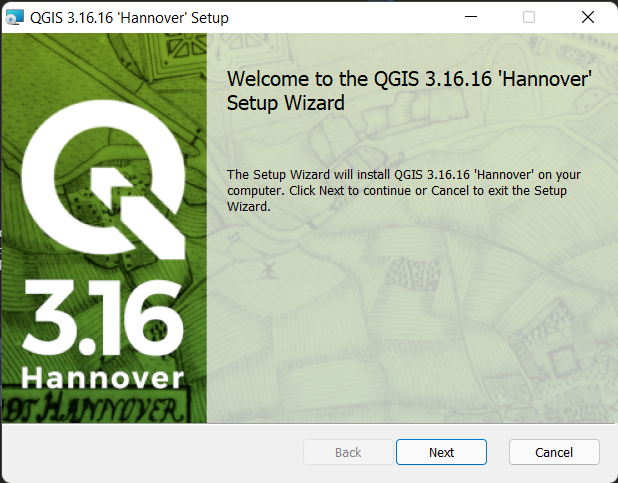
\includegraphics{images/Index0/win01.png}

На следующем шаге будет показано лицензионное соглашение QGIS и другого программного обеспечения, входящего в пакет поставки. Нажмите «Принимаю».

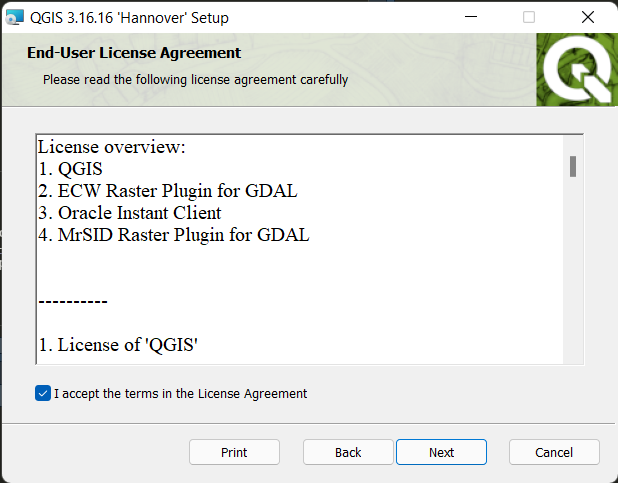
\includegraphics{images/Index0/win02.png}

На следующем шаге выберите папку для установки и отметьте, нужно ли создавать ярлыки на рабочем столе и в меню «Пуск». По возможности используйте параметры, предлагаемые по умолчанию.

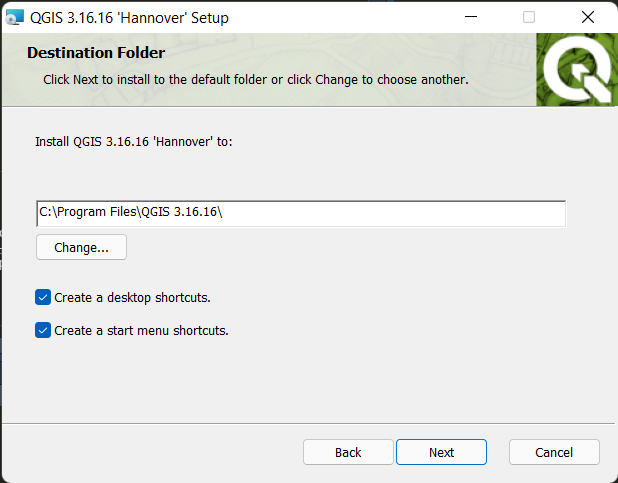
\includegraphics{images/Index0/win03.png}

На следующем шаге предлагается запустить процедуру установки. Нажмите «Install». Когда система выдаст запрос на внесение изменений, примите его.

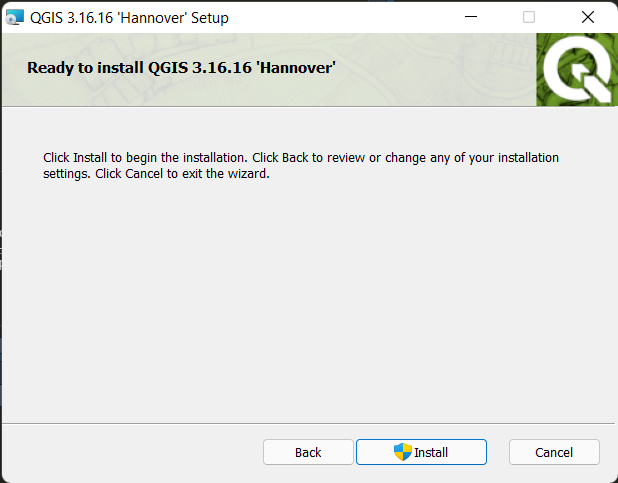
\includegraphics{images/Index0/win04.png}

После окончания установки ярлыки QGIS будут добавлены в меню «Пуск» и в отдельную папку QGIS на рабочем столе.

\hypertarget{macos}{%
\subsection*{macOS}\label{macos}}
\addcontentsline{toc}{subsection}{macOS}

По состоянию на 2024-06-25 для прохождения практикума рекомендуется использовать альтернативную сборку версии \href{https://www.kyngchaos.com/files/software/qgis/QGIS-macOS-3.4.12-1.dmg}{3.4.12}. Перейдя по ссылке, необходимо согласиться сохранить образ установочного диска на компьютер (можно разрешить его сразу открыть средствами \emph{DiskImageMounter}):

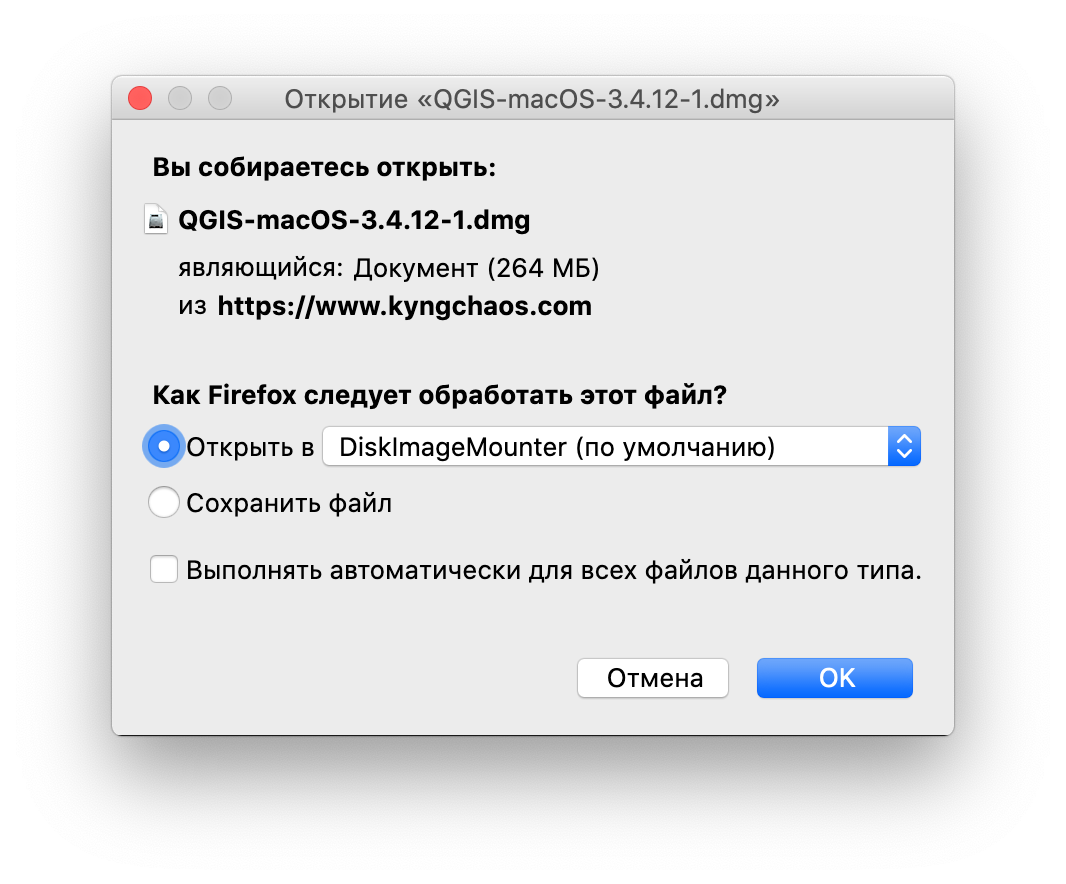
\includegraphics{images/Index0/mac01.png}

После того как образ загрузится и будет открыт, необходимо последовательно запустить три установщика, выделенные на снимке экрана ниже (именно в том порядке, в котором они пронумерованы!):

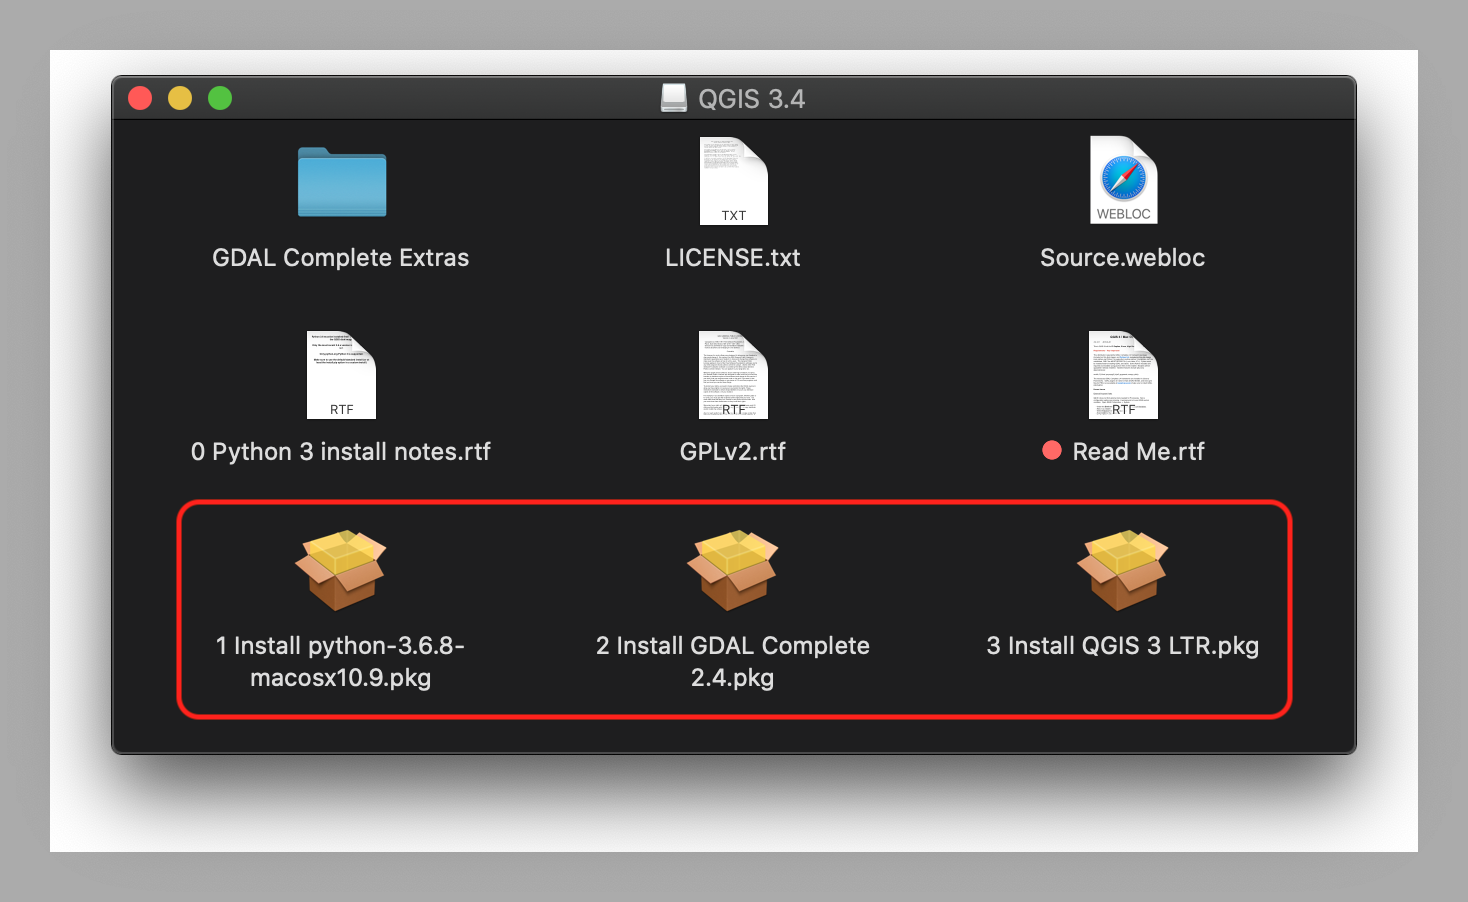
\includegraphics{images/Index0/mac02.png}

Установщики \textbf{GDAL Complete} и \textbf{QGIS 3 LTR} необходимо запускать через контекстное меню и выбирать пункт «Открыть»:

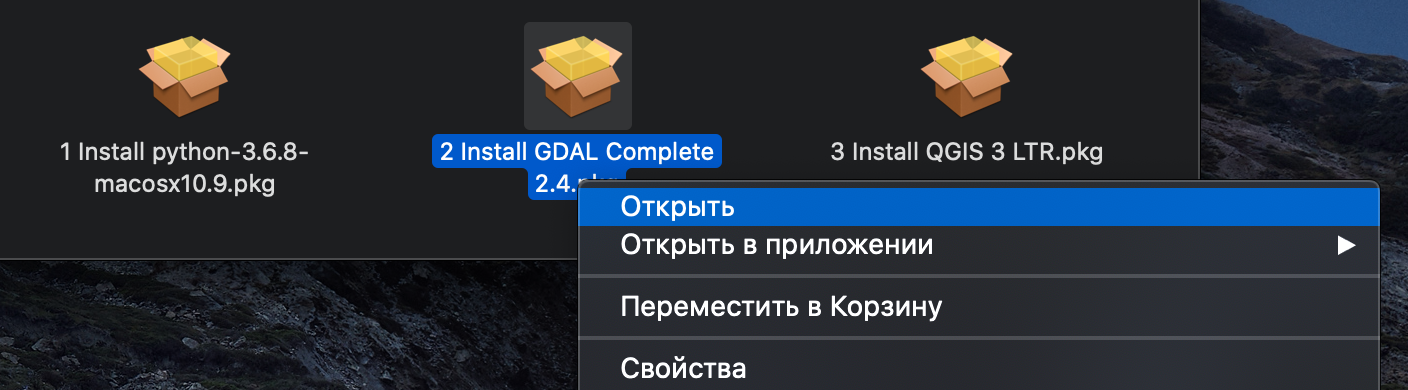
\includegraphics{images/Index0/mac03.png}

В появившемся диалоговом окне необходимо нажать «Открыть», чтобы разрешить установку:

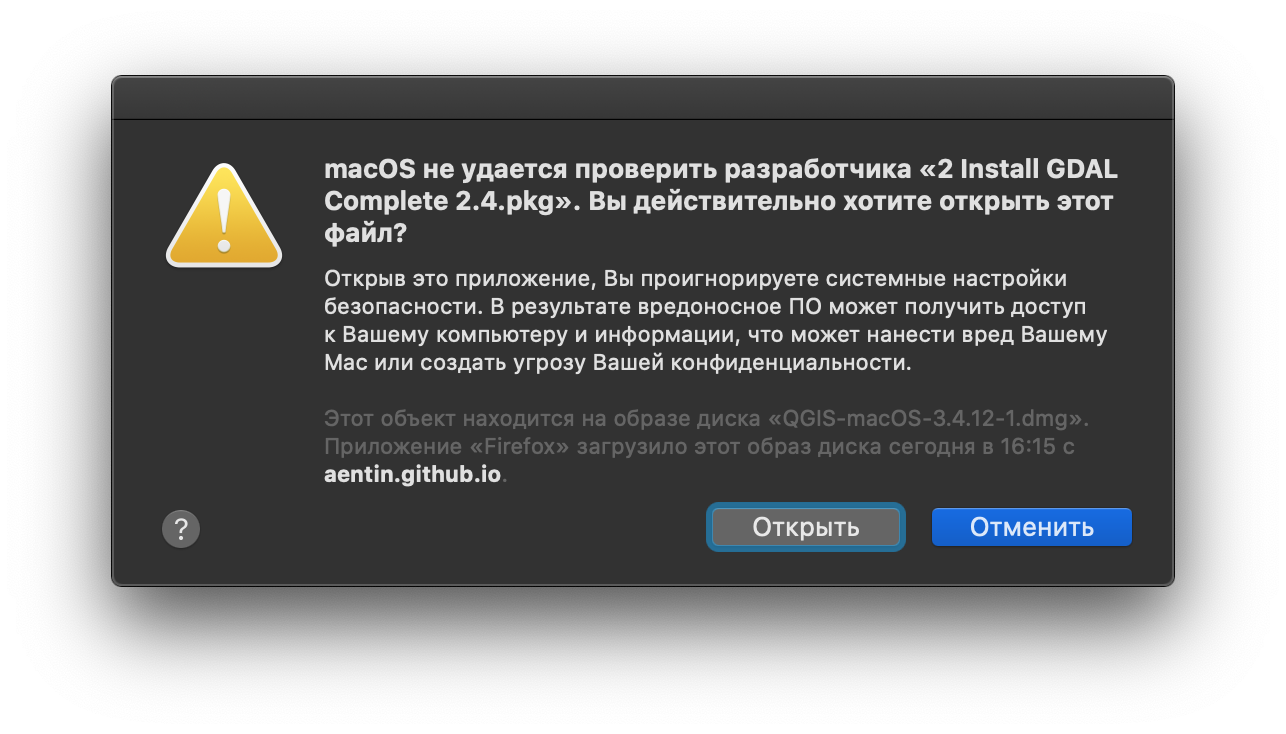
\includegraphics{images/Index0/mac04.png}

Все опции при установке каждой компоненты приложения оставляйте по умолчанию, ничего не меняйте и нажимайте в диалоговых окнах «Продолжить», пока не запустится установщик.

После того как последняя компонента --- \textbf{QGIS} --- будет установлена, вы сможете найти приложение и запустить его из каталога \emph{Программы} macOS:

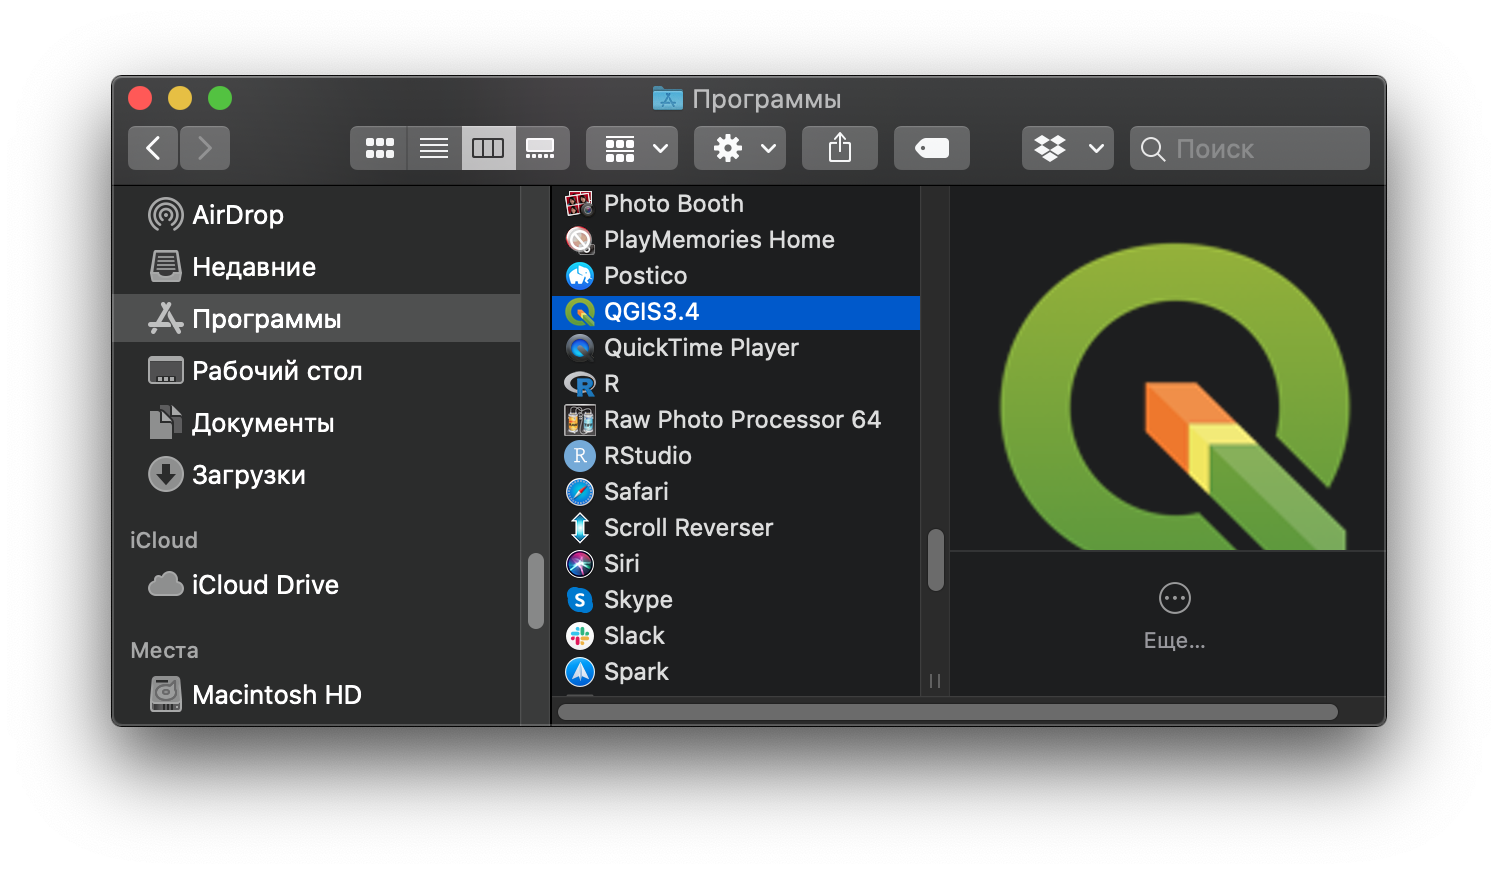
\includegraphics{images/Index0/mac05.png}

\hypertarget{linux}{%
\subsection*{Linux}\label{linux}}
\addcontentsline{toc}{subsection}{Linux}

Воспользуйтесь инструкциями по \href{https://qgis.org/ru/site/forusers/alldownloads.html\#linux}{этой ссылке}.

Дополнительную информацию по установке можно найти на \url{https://qgis.org/ru/site/forusers/download.html}.

\hypertarget{global}{%
\section{Изменение языка интерфейса и прочих глобальных переменных QGIS}\label{global}}

В справке используется англоязычная версия QGIS. Чтобы поменять язык интерфейса в меню основного окна QGIS выберите \textbf{Установки -- Параметры} (\textbf{Settings -- Options})

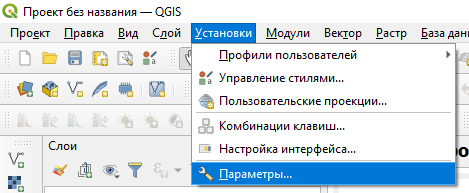
\includegraphics{images/Index0/Options.png}

В разделе \textbf{Общие улучшения} (\textbf{General}) поставьте галочку возле пункта \textbf{Переопределить языковые настройки} (\textbf{Override system locale}) и выберите напротив пункта \textbf{Перевод пользовательского интерфейса} (\textbf{User interface translation}) язык \textbf{American English}. Нажмите на кнопку \textbf{OK}. Изменения вступят в силу после перезагрузки QGIS.

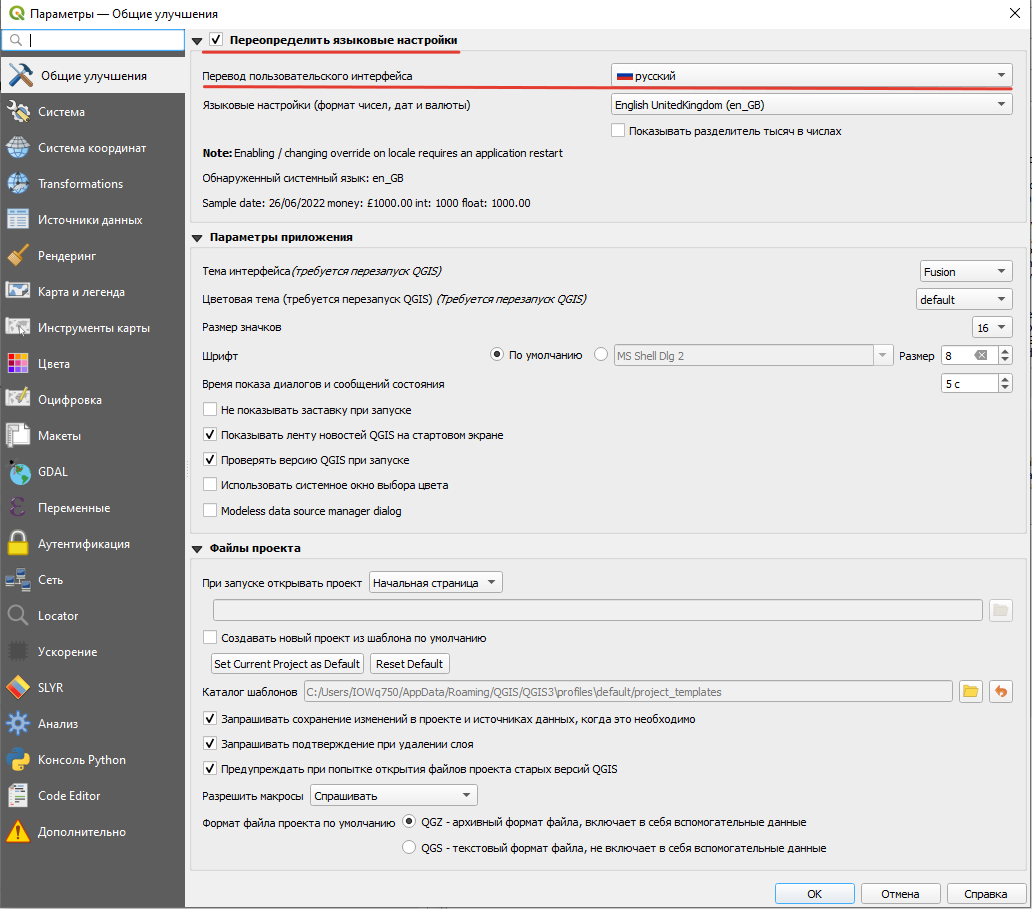
\includegraphics{images/Index0/Interface.png}

\begin{longtable}[]{@{}l@{}}
\toprule\noalign{}
\endhead
\bottomrule\noalign{}
\endlastfoot
\emph{Карпачевский А.М.} \textbf{Основы дистанционного зондирования и фотограмметрии}. М.: Географический факультет МГУ, 2024. \\
\end{longtable}

\hypertarget{pansharpen}{%
\chapter{Преобразования пространственного разрешения}\label{pansharpen}}

\hypertarget{pansharpen-project}{%
\section{Создание проекта в ArcGIS Pro}\label{pansharpen-project}}

Запустите ArcGIS Pro. В открывшемся окне выберите запуск проекта без шаблона.

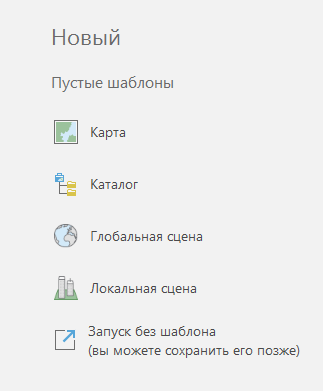
\includegraphics{images/Ref01/Launching.png}

Окно программы состоит из нескольких основных панелей: слева таблица содержания, самое большое окно посередине -- окно карты, справа панель каталог и инструментов геообработки. Панель каталога нужна для того чтобы обращаться к данным, расположенным на компьютере. Раскройте пункт \textbf{Folders} и найдите свою папку, либо папку, расположенную выше по древу. Если её нет, можно добавить подключение к папке, щёлкнув правой кнопкой мыши.

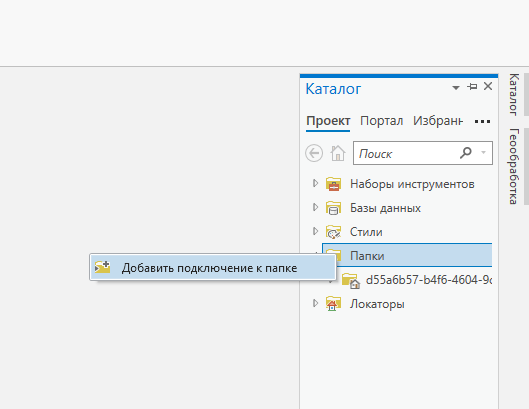
\includegraphics{images/Ref01/Add_Connection.png}

Внутри своей папки создайте новую базу геоданных, щёлкнув по ней правой кнопкой.

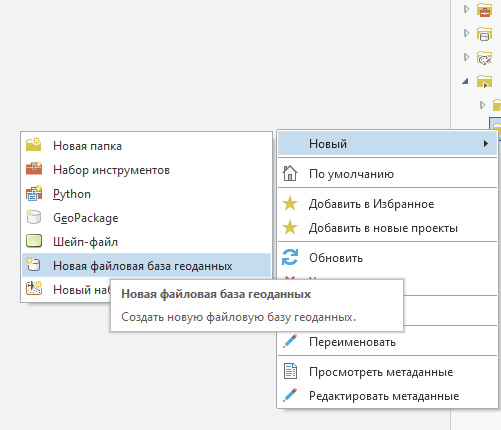
\includegraphics{images/Ref01/New_GDB.png}

После этого база геоданных появится в перечне всех доступных баз данных в каталоге. Найдите там свою базу и сделайте её базой по умолчанию.

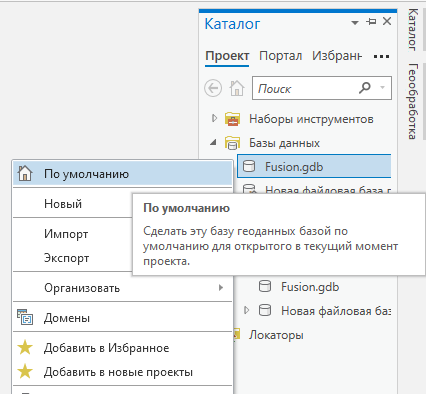
\includegraphics{images/Ref01/Default.png}

Через главное меню добавьте новую карту.

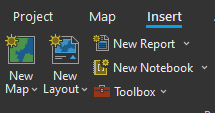
\includegraphics{images/Ref01/New_Map.png}

Сохраните проект
\includegraphics{images/Ref01/Save_Project.png} в той же директории, где расположена база данных, после чего в каталоге на этой папке должен появиться значок домика.

\hypertarget{pansharpen-composite}{%
\section{Создание композита}\label{pansharpen-composite}}

Для создания композита перетащите из окна каталога файлы отдельных каналов изображения. В панели геообработки найдите набор инструментов \textbf{Data Management Tools -- Raster -- Raster Processing}, внутри него выберите инструмент \textbf{Composite Band}.

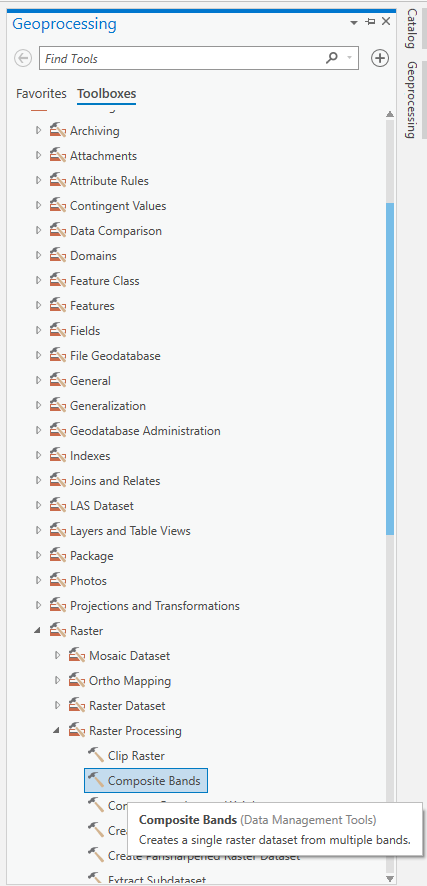
\includegraphics{images/Ref01/Raster_tools.png}

На вход инструменту подайте отдельные каналы, на выход укажите название итогового композита -- обратите внимание, что он должен быть в базе геоданных по умолчанию.

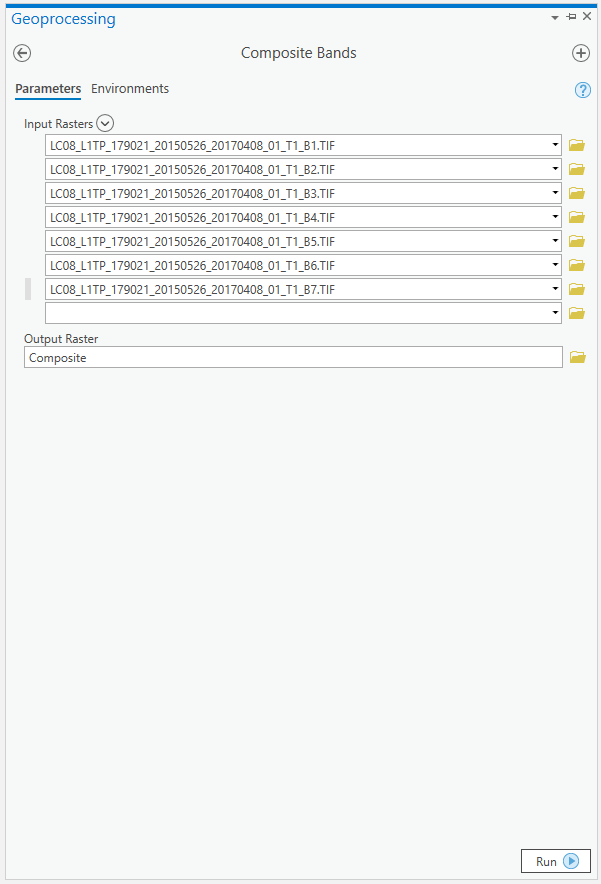
\includegraphics{images/Ref01/Composite_bands.png}

Для того чтобы задать визуализацию синтеза каналов нового композита, выделите слой и перейдите во вкладку \textbf{Appearance} основной ленты меню. В \textbf{Band Combination} укажите пользовательский синтез (\textbf{Custom}) и задайте соответствие каналов изображения каналам основных цветов.

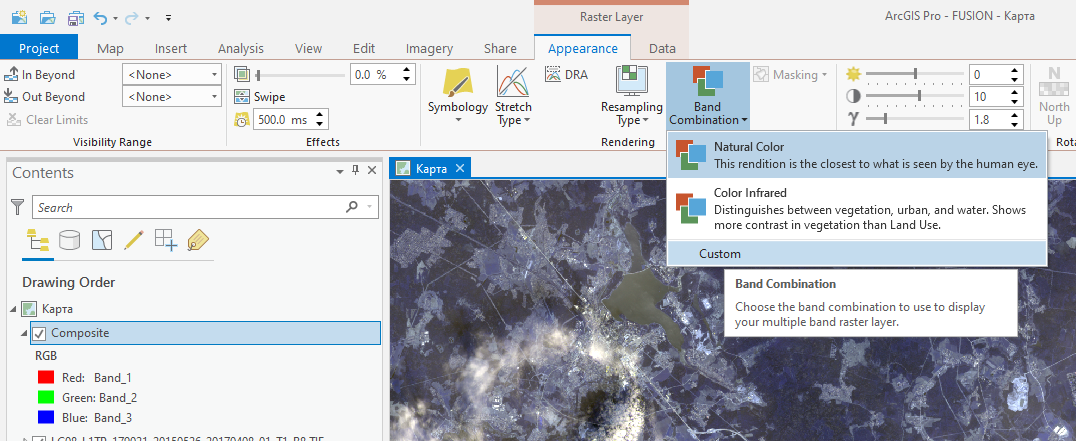
\includegraphics{images/Ref01/Band_combination.png}

\hypertarget{pansharpen-extract}{%
\section{Вырезание фрагмента изображения}\label{pansharpen-extract}}

Для вырезания фрагмента изображения необходимо создать новый класс объектов в базе геоданных. Для этого щёлкните правой кнопкой мыши по базе \textbf{New -- Feature Class}. В открывшемся окне задайте имя и систему координат класса.

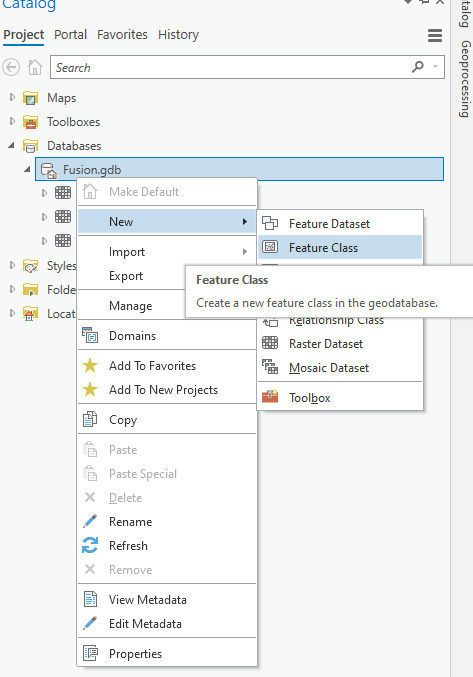
\includegraphics{images/Ref01/New_FC.png}

Добавьте класс объектов в окно карты и перейдите на вкладку \textbf{Edit} главного меню, выберите пункт \textbf{Create}.

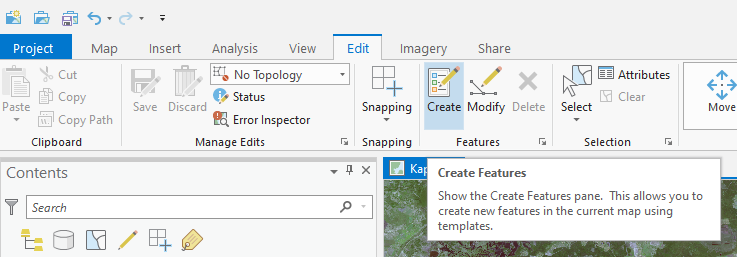
\includegraphics{images/Ref01/Create.png}

Справа откроется панель с шаблонами объектов. Выберите способ создания объекта -- прямоугольник. Отрисуйте прямоугольник на карте, который охватит вырезаемую область изображения.

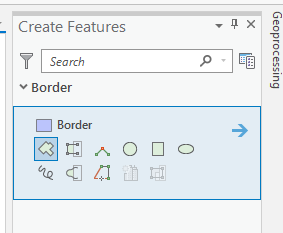
\includegraphics{images/Ref01/Rectangles.png}

После того, как объект будет готов, сохраните изменения, нажав на кнопку 
\includegraphics{images/Ref01/Save_edits.png}.

Вырезается фрагмент изображения с помощью инструмента \textbf{Extract by Mask} -- его можно найти на панели инструментов геообработки в наборе инструментов \textbf{Spatial Analyst Tools -- Extraction}.

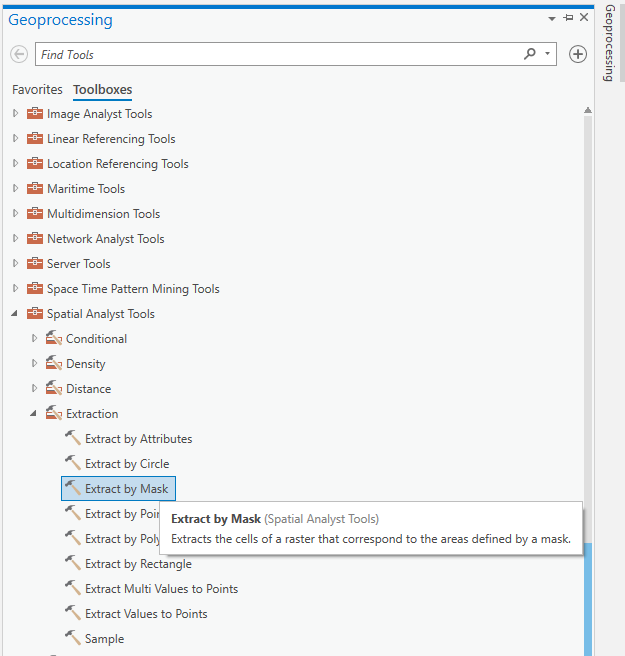
\includegraphics{images/Ref01/Extract_by_Mask.png}

У полученного фрагмента изображения может быть не настроена гистограмма. Перейдите во вкладку \textbf{Appearance} и нажмите на кнопку \textbf{DRA} для автоматической настройки гистограммы фрагмента, либо исправьте гистограмму вручную.

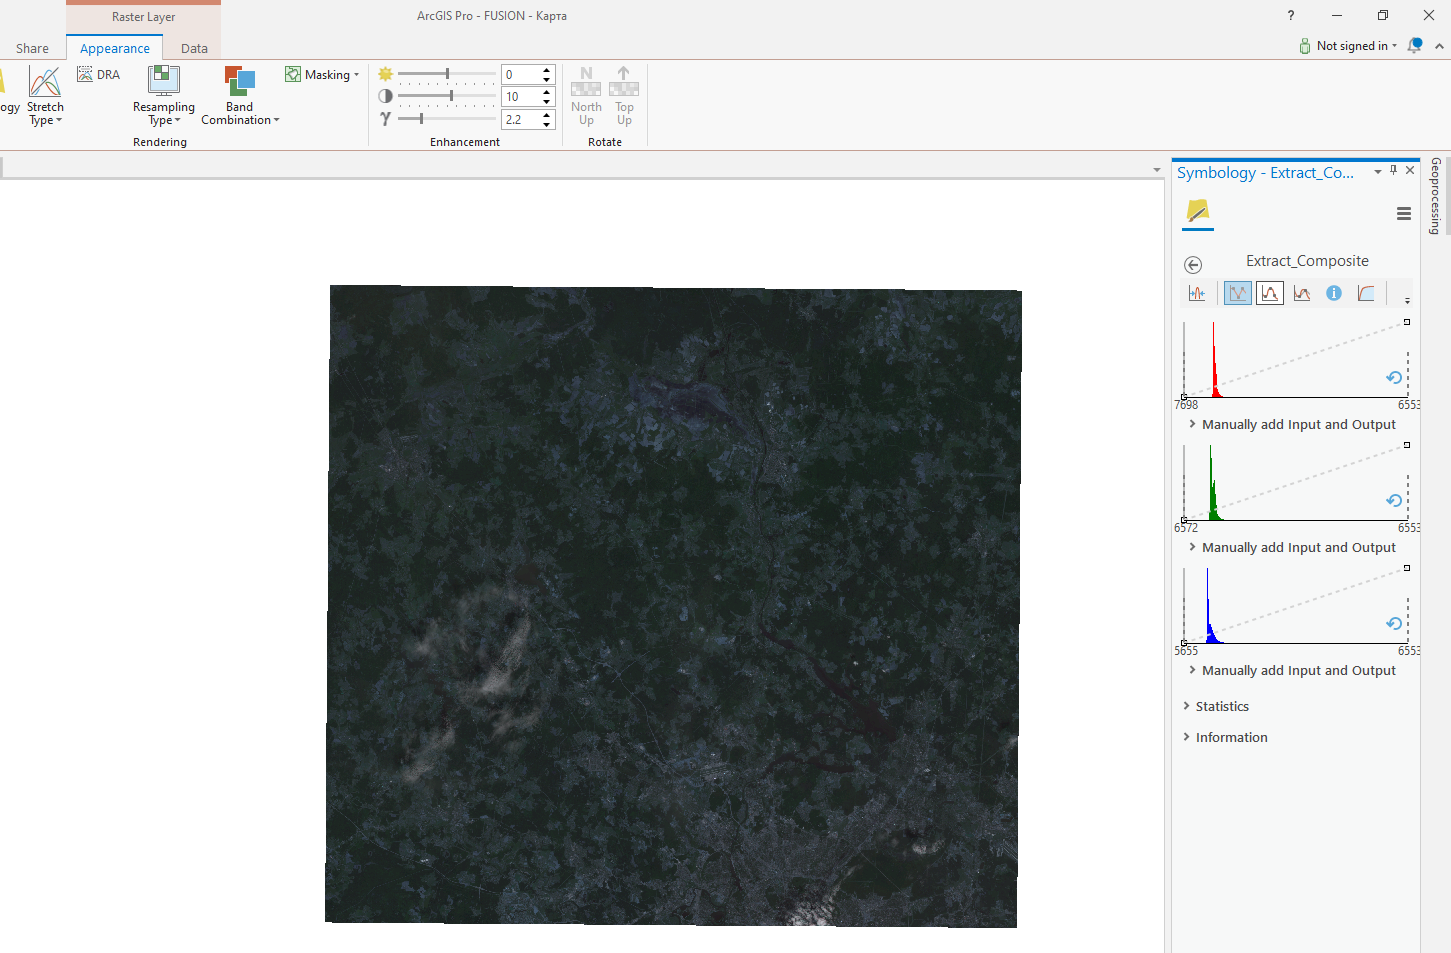
\includegraphics{images/Ref01/Stretching.png}

\hypertarget{pansharpen-filter}{%
\section{Фильтрация}\label{pansharpen-filter}}

Для градиентной фильтрации выберите растр, в основной ленте меню выберите вкладку \textbf{Imagery}, нажмите на кнопку \textbf{Raster Functions} -- у вас справа откроется панель с различными инструментами растров, в том числе во вкладке \textbf{Appearance} есть инструмент свёртки (\textbf{Convolution}).

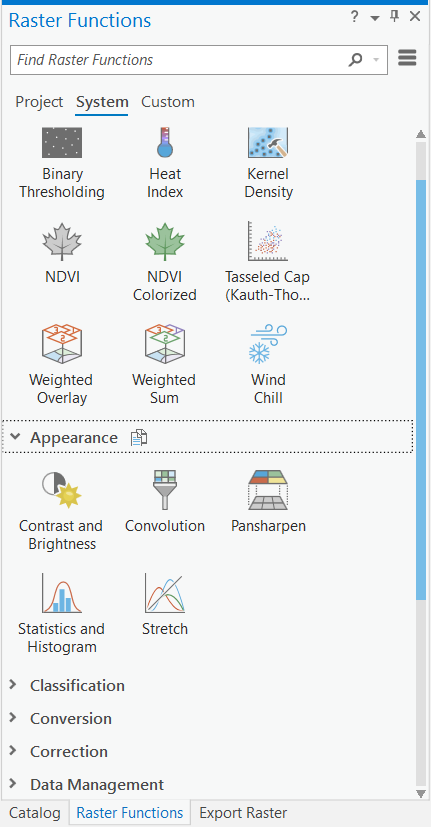
\includegraphics{images/Ref01/Raster_functions.png}

Для линейной (высокочастотная, низкочастотная) фильтрации можно использовать инструмент \textbf{Spatial Analyst Tools -- Neighborhood -- Filter}. В качестве входных параметров необходимо указать исходный растр, а также тип фильтрации.

\hypertarget{pansharpen-resampling}{%
\section{Передискретизация}\label{pansharpen-resampling}}

Для передискретизации используется инструмент \textbf{Data Management Tools -- Raster -- Raster Processing -- Resample}. В качестве входных параметров необходимо указать исходный растр, а также размер ячейки нового растра и тип интерполяции

\hypertarget{pansharpen-pansharpen}{%
\section{Паншарпенинг}\label{pansharpen-pansharpen}}

Для паншарпенинга используется инструмент \textbf{Data Management Tools -- Raster -- Raster Processing -- Create Pansharpened Raster Dataset}. В качестве входных параметров необходимо указать исходный растр, тип преобразования и некоторые другие параметры, которые зависят от типа преобразования.

\hypertarget{pansharpen-layout}{%
\section{Работа в режиме компоновки}\label{pansharpen-layout}}

Для работы с данными в ArcGIS Pro мы находимся в окне карты (\textbf{Map}). Вы можете создать несколько окон карты через меню \textbf{Insert -- New Map}. Слои содержания можно скопировать в каждую карту, а также синхронизировать их визуализацию через меню \textbf{View -- Link Views -- Center And Scale}. Создание компоновки осуществляется через меню \textbf{Insert -- New Layout}, после чего у вас откроются варианты с параметрами листа компоновки. Эти параметры, включая ориентировку листа можно поменять в свойствах, вызвав их нажатием правой кнопки мыши.

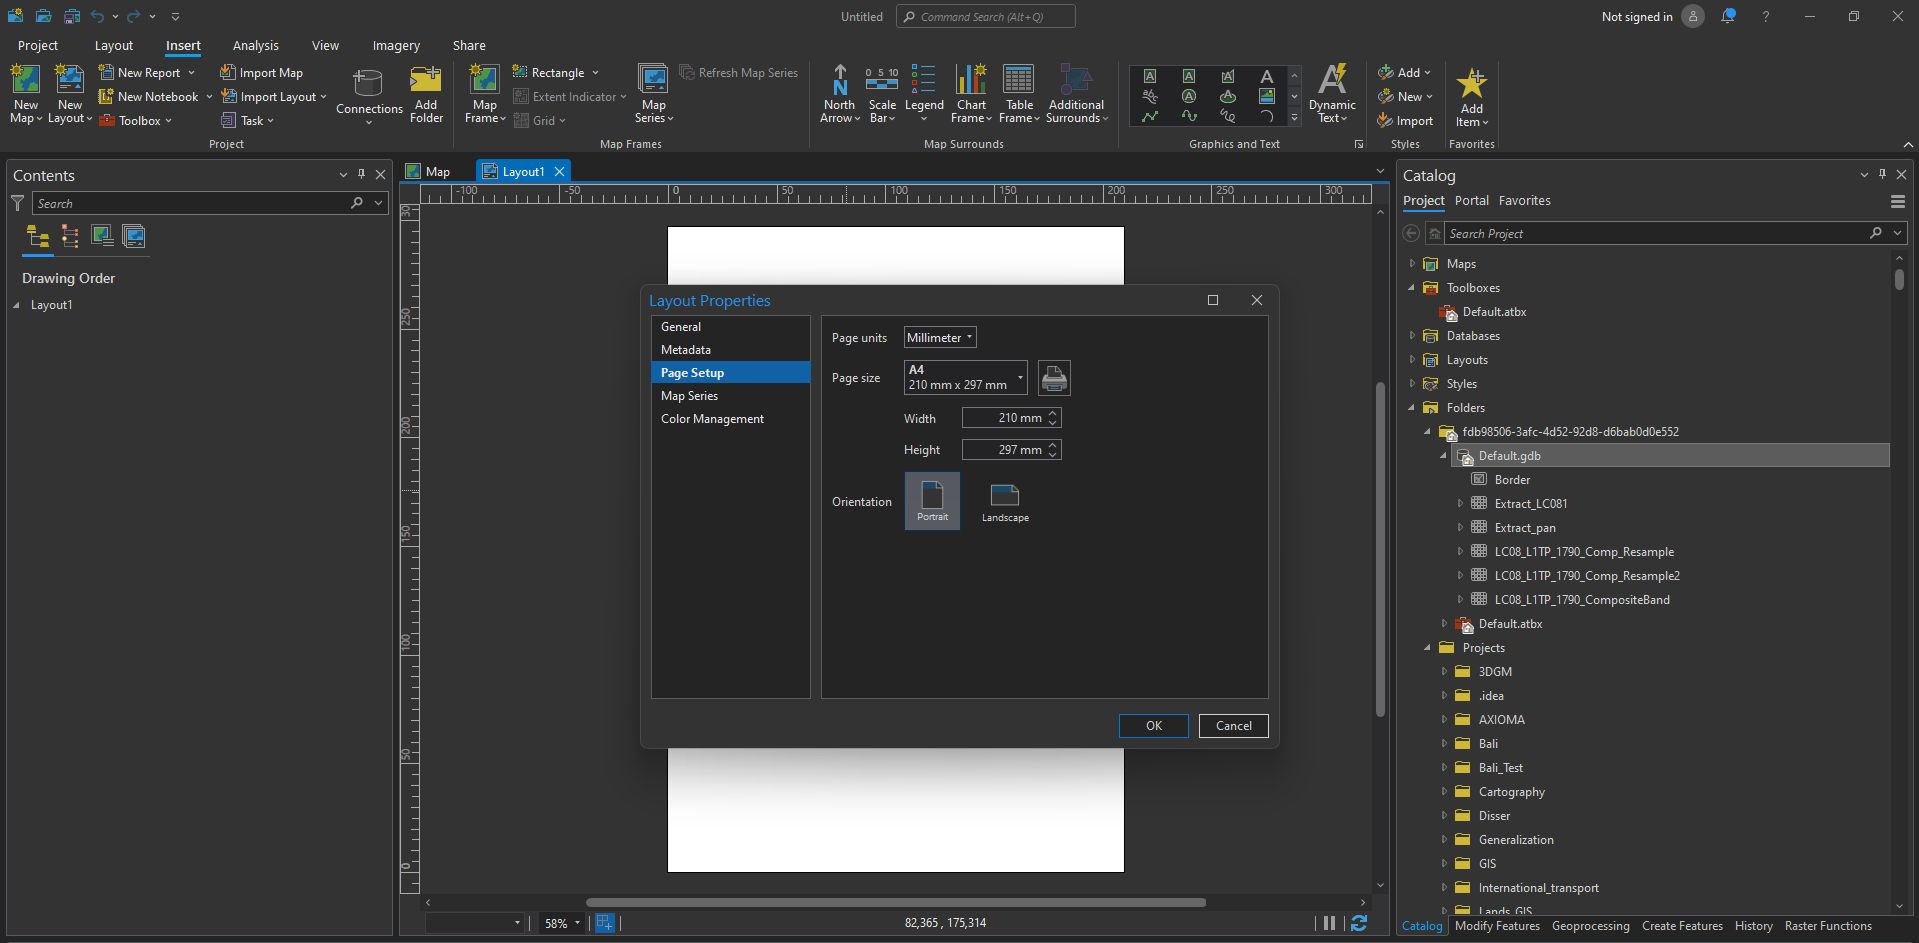
\includegraphics{images/Ref01/Layout_Properties.png}

Используйте кнопку \textbf{Insert -- Map Frame} для того чтобы вставить картографическое изображение в лист компоновки.На одном листе можно разместить несколько картографических изображений, последовательно используя эту кнопку. Выделенный фрейм карты будет жирным в таблице содержания и отображаться в режиме узлов на листе карты.

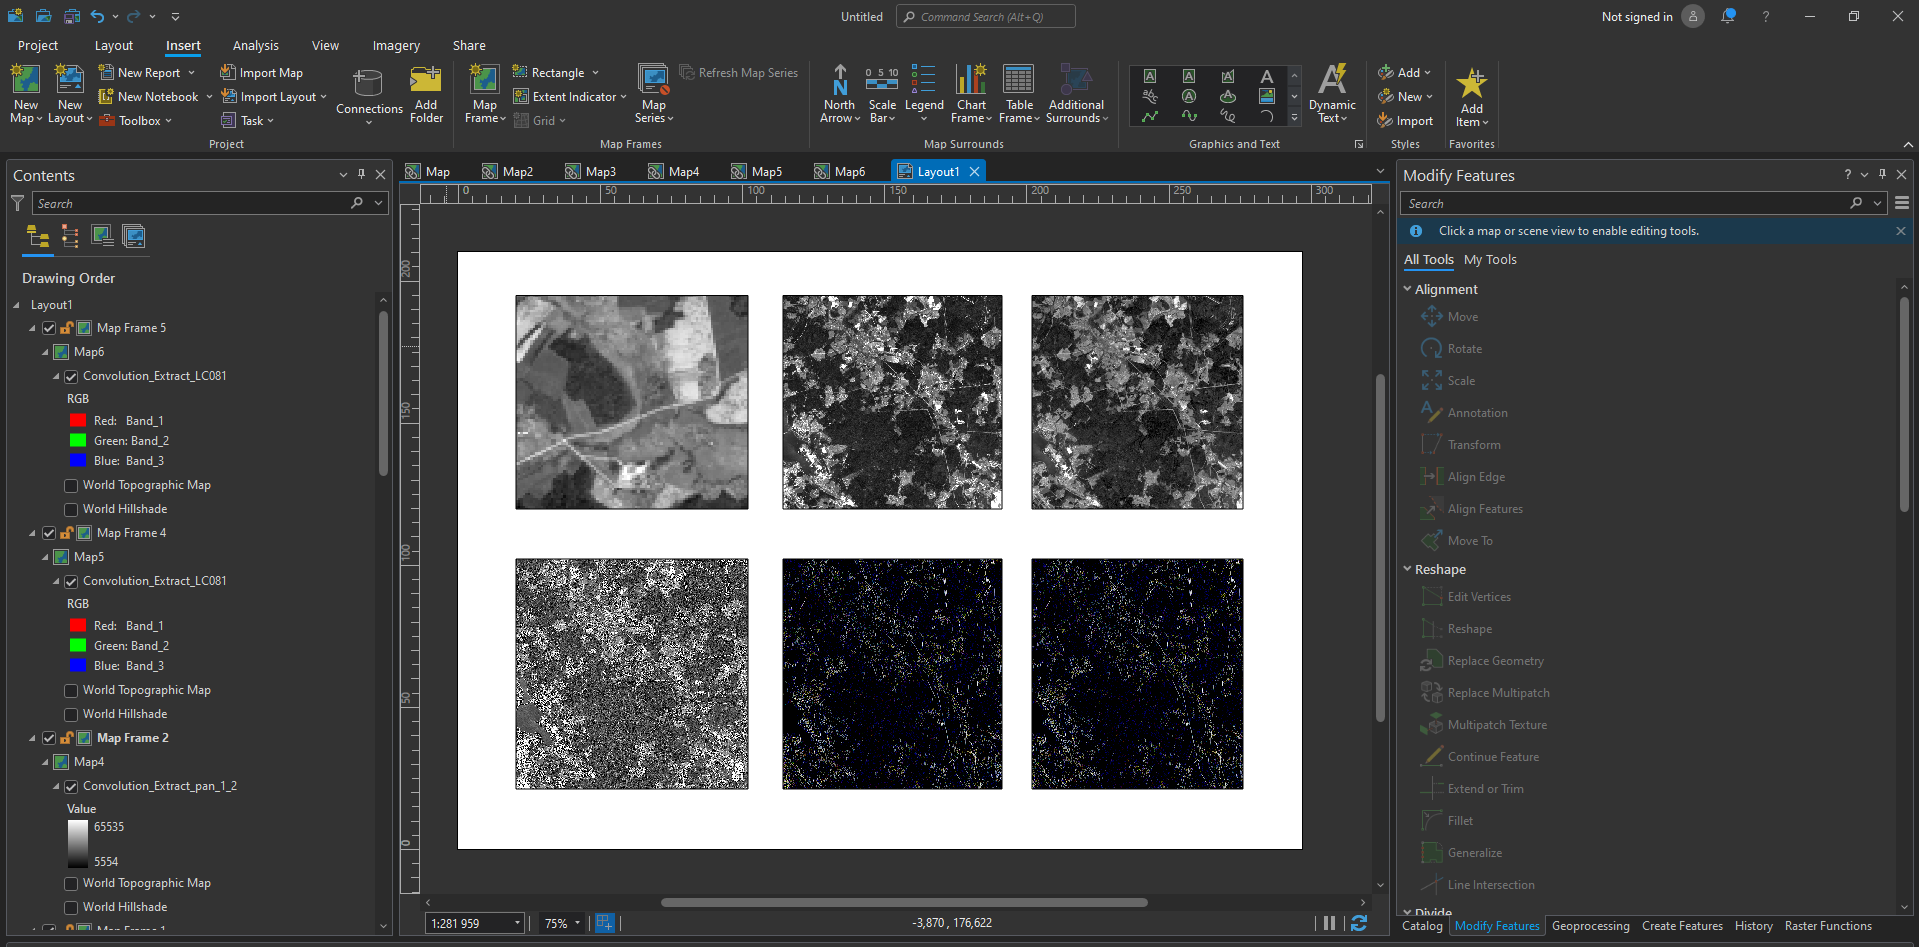
\includegraphics{images/Ref01/Map_Frames.png}

Для того чтобы область охвата фрейма переместилася к вашим данным, выберите соответствующий слой в таблице содержания и правой кнопкой вызовите меню \textbf{Zoom To Layer}. Вы можете менять масштаб изображения внутри фрейма в соответствующем окошке внизу. Для перемещения данных в пределах окна фрейма необходимо активировать карту правой кнопкой мыши и нажав \textbf{Activate}. Затем вернитесь в меню \textbf{Map} и переключитесь в режим \textbf{Explore}. Для выхода обратно в режим компоновки нажмите \textbf{Close Activation}.

\includegraphics{images/Ref01/Map_Frame_Activation.gif}

Для всех фреймов можно выставить экстент из окна карты \textbf{Layout -- Zoom To Map View} или \textbf{Layout -- Zoom To Last Active View}.

В окно компоновки можно вставить другие элементы: текст, графику, масштабную линейку и т.д. Правой кнопкой можно зайти в свойства элемента, поменять гарнитуру, кегль, выравнивание и прочие параметры.

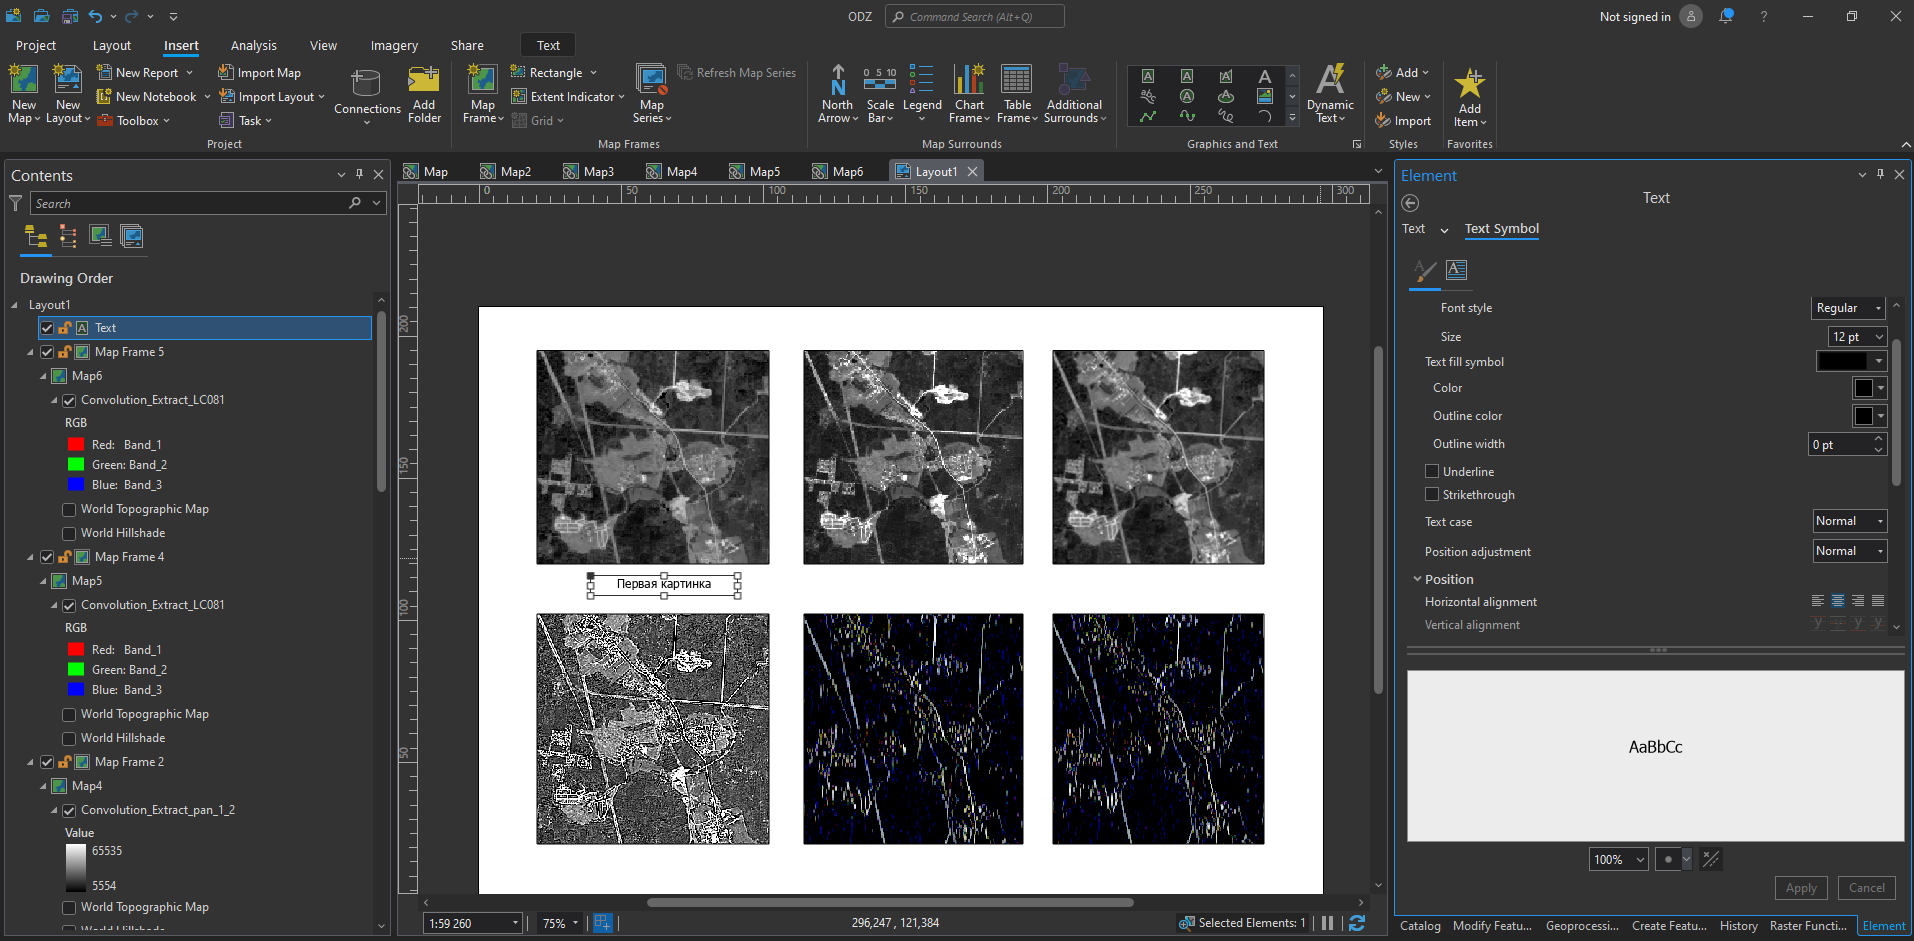
\includegraphics{images/Ref01/Graphic_Elements.png}

Экспорт составленного макета компоновки можно сделать через меню \textbf{Share -- Export Layout} или скопировать изображение в буфер обмена \textbf{Capture To Clipboard}

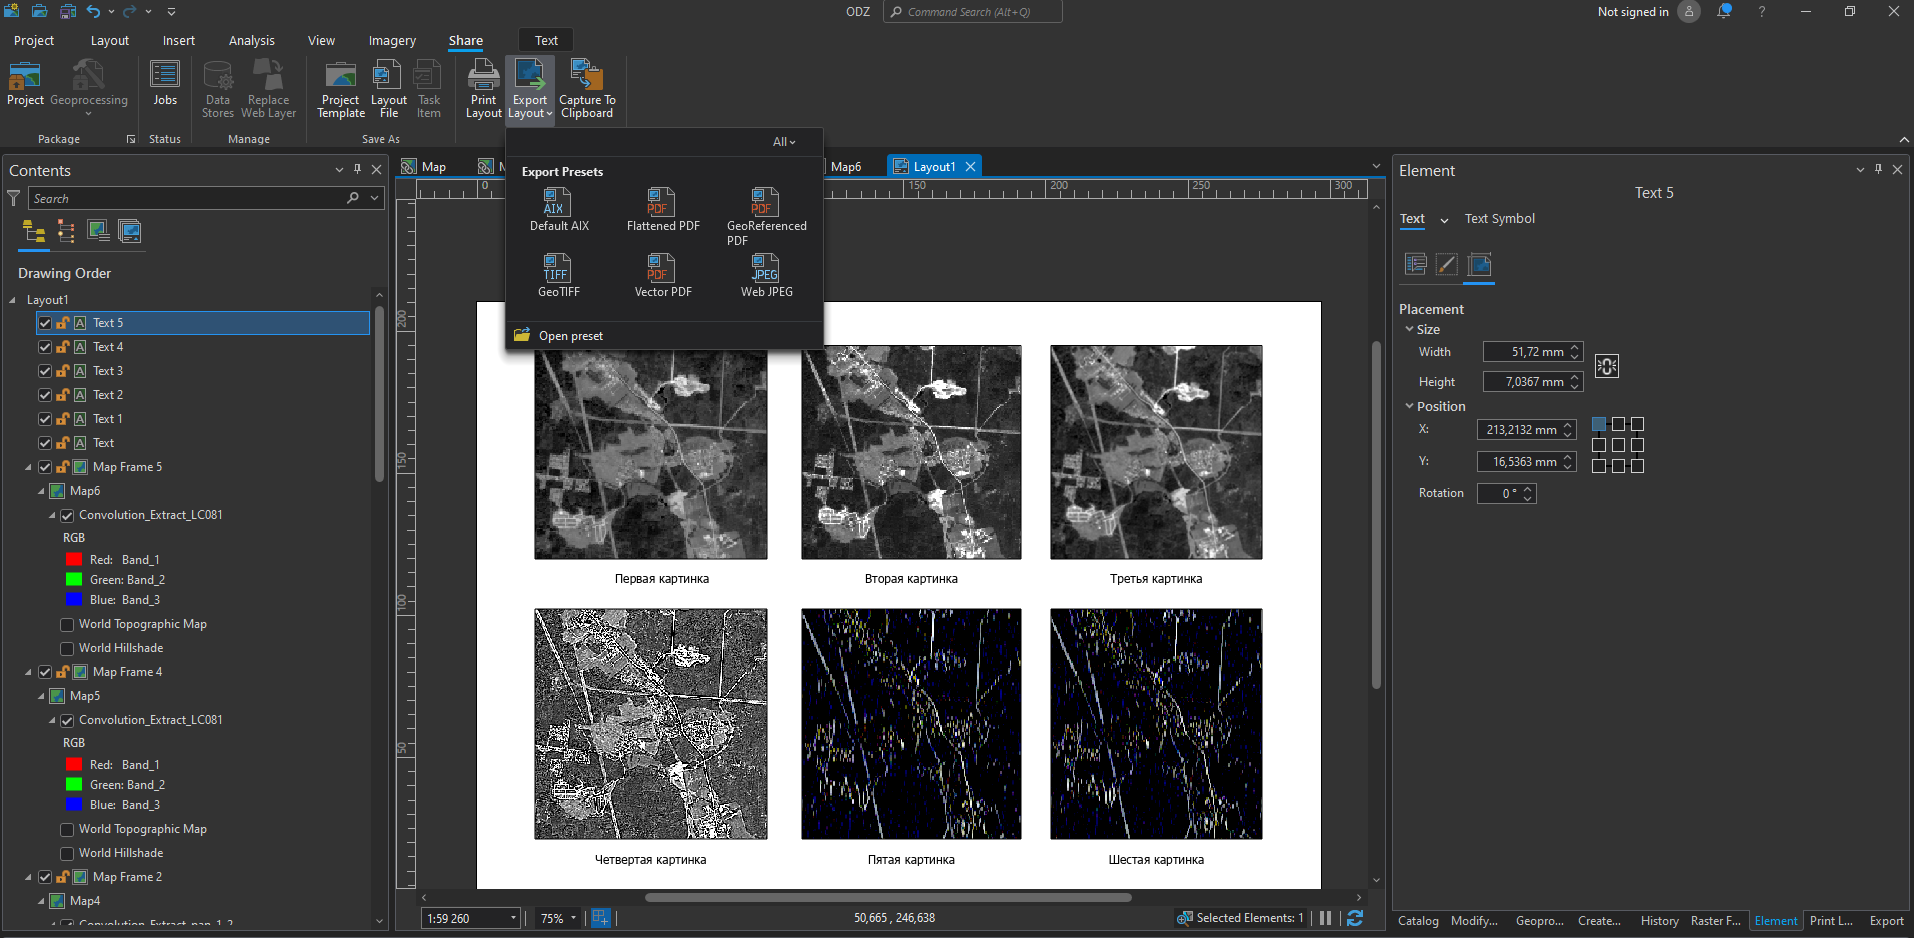
\includegraphics{images/Ref01/Export.png}

\begin{longtable}[]{@{}l@{}}
\toprule\noalign{}
\endhead
\bottomrule\noalign{}
\endlastfoot
\emph{Карпачевский А.М.} \textbf{Основы дистанционного зондирования и фотограмметрии}. М.: Географический факультет МГУ, 2024. \\
\end{longtable}

\hypertarget{georeference}{%
\chapter{Географическая привязка}\label{georeference}}

\hypertarget{georeference-arcgis}{%
\section{Географическая привязка в ArcGIS Pro}\label{georeference-arcgis}}

\hypertarget{ux43fux440ux438ux432ux44fux437ux43aux430-ux43dux430-ux43eux441ux43dux43eux432ux435-ux432ux432ux43eux434ux430-ux43aux43eux43eux440ux434ux438ux43dux430ux442}{%
\subsection{Привязка на основе ввода координат}\label{ux43fux440ux438ux432ux44fux437ux43aux430-ux43dux430-ux43eux441ux43dux43eux432ux435-ux432ux432ux43eux434ux430-ux43aux43eux43eux440ux434ux438ux43dux430ux442}}

Создайте новый проект и сохраните его. Задайте систему координат датафрейма (карты) -- для этого зайдите в свойства \textbf{Map} и перейдите во вкладку \textbf{Coordinate Systems}, раскройте список \textbf{Projected coordinate system} и выберите нужную СК.

\begin{figure}
\centering
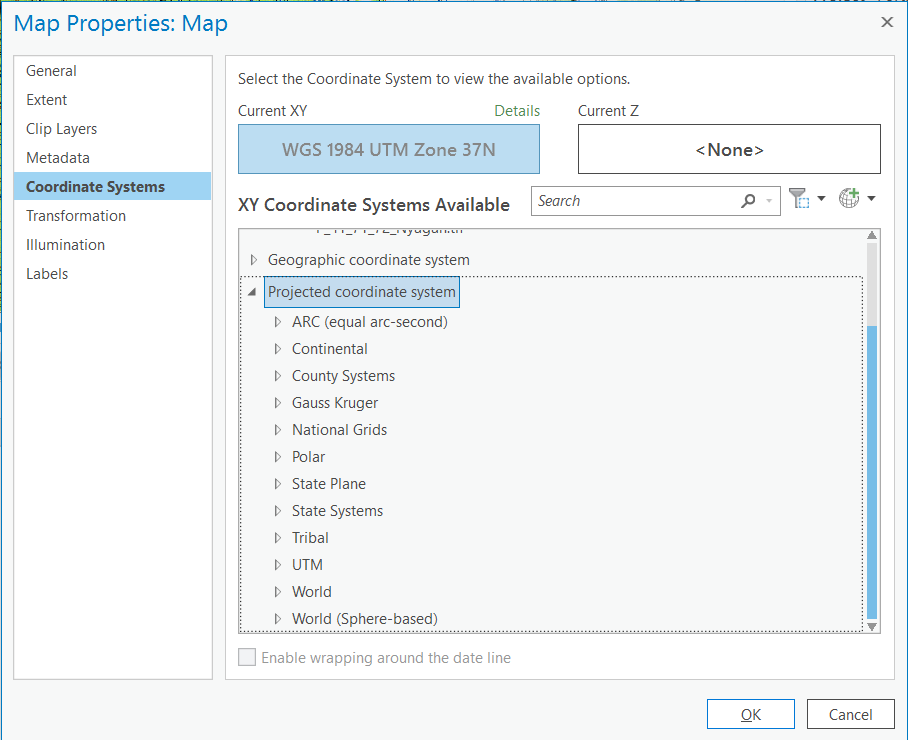
\includegraphics{images/Ref02/Arc_mapCRS.png}
\caption{Свойства системы координат карты}
\end{figure}

Добавьте из панели каталога растр, который необходимо привязать.Выделите его в списке слоев и во вкладке \textbf{Imagery} нажмите на кнопку \textbf{Georeference}.

\begin{figure}
\centering
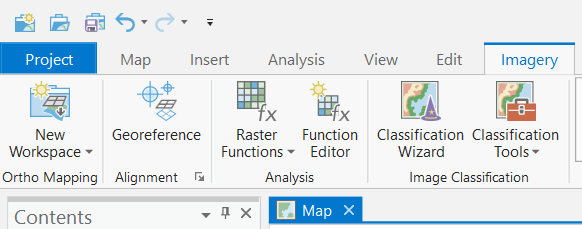
\includegraphics{images/Ref02/Arc_georeference.png}
\caption{Открытие панели привязки}
\end{figure}

Открытая панель привязки состоит из нескольких кнопок. Убедитесь, что у вас нажата кнопка \textbf{Auto Apply}, которая позволяет трансформировать изображение на лету.

\begin{figure}
\centering
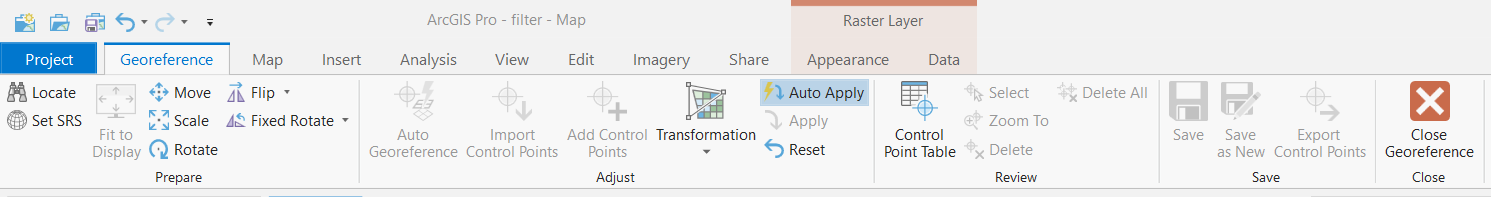
\includegraphics{images/Ref02/Arc_georef_panel.png}
\caption{Панель привязки}
\end{figure}

Нажмите на кнопку \textbf{Add Control Points} 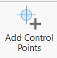
\includegraphics{images/Ref02/Arc_add_control_points.png} и установите опорную точку в нужном месте на карте. После этого вам будет предложено установить соответственную точку на референцном слое или ввести заданные координаты для точки -- для этого щёлкните правой кнопкой мыши, после чего откроется окошко для ввода координат.

\begin{figure}
\centering
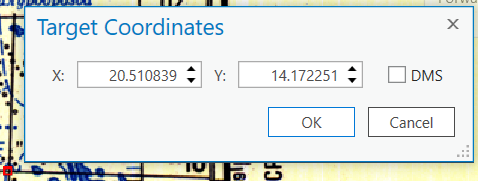
\includegraphics{images/Ref02/Arc_target_coords.png}
\caption{Окно ввода координат опорной точки}
\end{figure}

Если нажать на кнопку \textbf{Control Point Table} 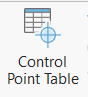
\includegraphics{images/Ref02/Arc_control_points_tab.png}, то откроется таблица, где будут показаны все установленные опорные точки с их координатами в исходной и референцной системе координат. В этой же таблице указываются ошибки (невязки) общая и по отдельным координатам. Слева можно включать и выключать точки из расчёта. Когда точка выключена из расчёта, она превращается из опорной в контрольную.

\begin{figure}
\centering
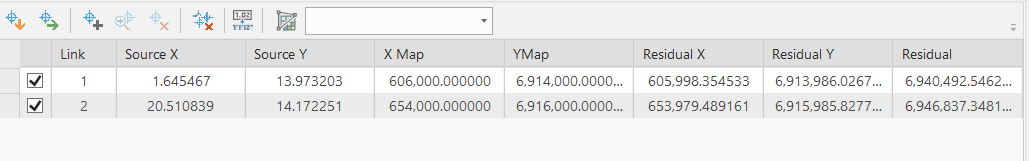
\includegraphics{images/Ref02/Arc_table.png}
\caption{Таблица координат опорных точек}
\end{figure}

Установив необходимое количество точек, вы можете нажать на кнопку \textbf{Transformation} 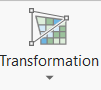
\includegraphics{images/Ref02/Arc_transformation.png}и выбрать тип трансформации. После установки опорных точек и выбора типа трансформации можно запустить процесс трансформирования и сохранения нового изображения, нажав на кнопку 
\includegraphics{images/Ref02/Arc_save_as_new.png}. При сохранении укажите путь внутрь базы данных, название для слоя, убедитесь в том, что разрешение выходного растра составляет 30 на 30, а также укажите глубину цветности \textbf{16} или \textbf{32 bit unsigned}.

\begin{figure}
\centering
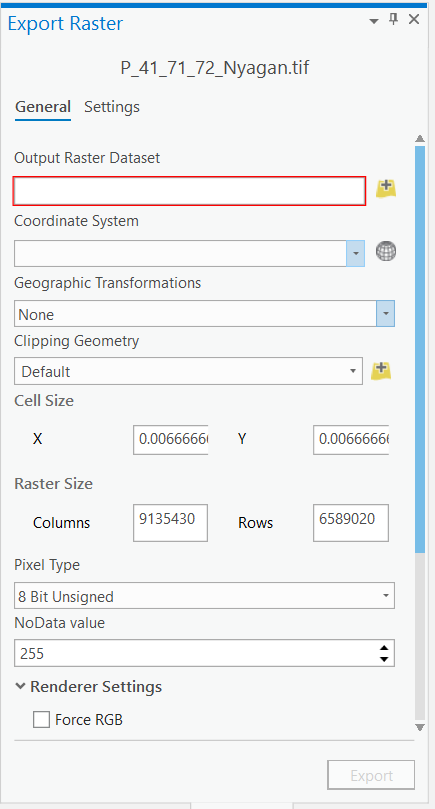
\includegraphics{images/Ref02/Arc_export_raster.png}
\caption{Окно сохранения трансформированного изображения}
\end{figure}

Обратите внимание, что опорные точки можно сохранять отдельно (экспортировать) -- для этого есть кнопка \textbf{Export Control Points} и импортировать \textbf{Import Control Points}.

\hypertarget{ux43fux440ux438ux432ux44fux437ux43aux430-ux43dux430-ux43eux441ux43dux43eux432ux435-ux440ux435ux444ux435ux440ux435ux43dux446ux43dux43eux433ux43e-ux438ux437ux43eux431ux440ux430ux436ux435ux43dux438ux44f}{%
\subsection{Привязка на основе референцного изображения}\label{ux43fux440ux438ux432ux44fux437ux43aux430-ux43dux430-ux43eux441ux43dux43eux432ux435-ux440ux435ux444ux435ux440ux435ux43dux446ux43dux43eux433ux43e-ux438ux437ux43eux431ux440ux430ux436ux435ux43dux438ux44f}}

При привязке снимка к референцному изображению удобно воспользоваться кнопкой \textbf{Fit to Display} 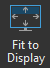
\includegraphics{images/Ref02/Arc_Fit_to_Display.png}, которая переместит привязывамаемое изображение в экстент, соответствующий текущему дисплею карты.

Далее для привязки неоходимо снова нажать на кнопку \textbf{Add Control Points} и поставить сначала точку на привязываемом изображении, а затем на референцном.

\begin{figure}
\centering
\includegraphics{images/Ref02/Arc_Image_to_Image.gif}
\caption{Привязка снимка к референцному изображению}
\end{figure}

К сожалению, в ArcGIS нет возможности сделать контрольные точки для оценки точности в данном модуле, но их можно создать искусственно. Для этого в окне каталога найдите свою базу данных или создайте новую. Внутри базы данных создайте точечный класс векторных объектов.

\begin{figure}
\centering
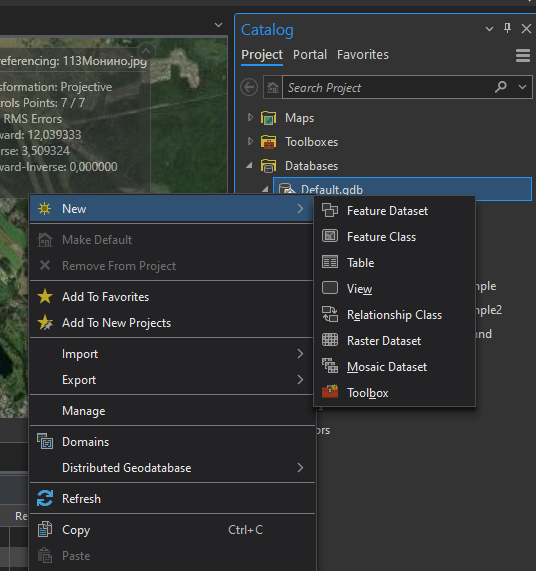
\includegraphics{images/Ref02/Arc_Create_FC.png}
\caption{Создание класса объектов}
\end{figure}

Задайте имя класса объекта латинскими буквами, без пробелов и спецсимволов, укажите тип геометрии -- \textbf{Point}, снимите галочку с координаты \textbf{Z}.

\begin{figure}
\centering
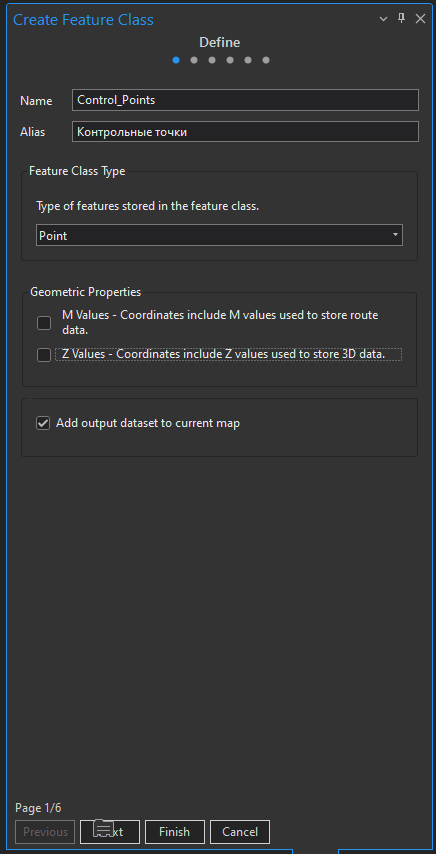
\includegraphics{images/Ref02/Arc_Create_Points.png}
\caption{Точечный класс объектов}
\end{figure}

Нас следующем шаге укажите целевую систему координат и нажмите на кнопку \textbf{Finish}.

Добавьте созданный класс объектов в качестве слоя на карту, если он не добавился автоматически. Выделите слой, перейдите на вкладку \textbf{Edit}, затем нажмите на кнопку \textbf{Create} и у вас откроется панель с шаблонами для создания векторных объектов. Выделите шаблон, нажмите на появившуюся под ним кнопку \textbf{Create point feature} и установите точку на референцном изображении. Сохраните изменения, нажав на кнопку \textbf{Save}.

\begin{figure}
\centering
\includegraphics{images/Ref02/Arc_Control_Points.gif}
\caption{Установка точек}
\end{figure}

Эти точки будут выступать в качестве реперов для оценки точности привязки. Для оценки отклонений их образа на привязываемом изображении перейдите на вкладку \textbf{Map}, возьмите линейку и измерьте расстояние от установленной точки до её предполагаемого положения на привязываемом изображении.

\begin{figure}
\centering
\includegraphics{images/Ref02/Arc_Measuring.gif}
\caption{Измерение отклонений}
\end{figure}

\hypertarget{georeference-qgis}{%
\section{Географическая привязка в QGIS}\label{georeference-qgis}}

\protect\hyperlink{georeference}{В начало справки ⇡}

Для привязки данных дистанционного зондирования в QGIS можно использовать WMS-сервис с мозаикой спутниковых снимков. Для включения мозаики зайдите в меню \textbf{Модули -- Управление и установка модулей\ldots{}}. Впишите в строку поиска \textbf{QuickMapServices}. Установите модуль.

Откроется окно модуля. В окне поиска геосервиса введите \textbf{Google satelite} или какой-либо еще картографический веб-сервис со спутниковой подложкой. Нажмите \textbf{Добавить}.

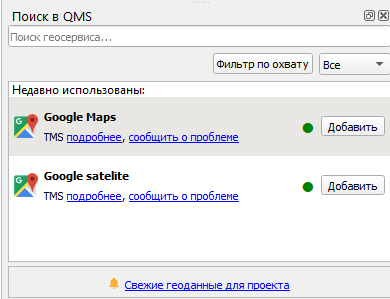
\includegraphics{images/Ref02/QMS.png}

Добавьте в качестве слоя данных привязываемый снимок.

В меню \textbf{Layers} найдите пункт \textbf{Referencer} 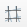
\includegraphics{images/Ref02/Reference_button.png}.

Откроется окно привязки. Нажмите на кнопку \textbf{Open Raster} \includegraphics{images/Ref02/Open_rastr.png}, добавьте привязываемый растр. Щелчок левой кнопкой мыши по привязываемому изображению открое окно, куда будет предложено ввести координаты. Если вы для привязки хотите использовать референцное изображение, нажмите на кнопку \textbf{С карты}.

\begin{figure}
\centering
\includegraphics{images/Ref02/Input_coordinates.png}
\caption{Окно ввода координат}
\end{figure}

Для настройки параметров трансформации нажмите на кнопку \includegraphics{images/Ref02/Transformation_settings.png}. Опорные точки можно сохранять и подгружать -- для этого используйте соответствующие кнопки на панели. Для запуска процесса трансформации нажмите на кнопку \includegraphics{images/Ref02/Transformation_button.png}

После добавления трансформированного изображения в основное окно карты убедитесь в правильности проделанной операции, сравнивая его с подложкой из мозаики спутниковых снимков. Для этого удобно использовать инструмент шторки.

Зайдите в \textbf{Модули -- Управление и установка модулей\ldots{}} и вбейте в поиск \textbf{MapSwipe Tool}. После этого появится панель шторки.

Выберите слой, который будет активен в режиме шторки (будет находиться под шторкой) и нажмите на кнопку \includegraphics{images/Ref02/Swipe_button.png}.

\begin{figure}
\centering
\includegraphics{images/Ref02/Swipe.png}
\caption{Режим шторки для слоя Google Maps}
\end{figure}

Установите опорные точки. Внизу окна появится таблица с вашими точками привязки -- будут указаны координаты этих точек в исходной СК изображения и в целевой СК, а также невязки. Далее необходимо указать способ трансформации для расчёта невязок. Нажмите на кнопку \includegraphics{images/Ref02/Transformation_settings.png}. В качестве типа трансформации для топографических карт должно быть достаточно полиномиального первой степени. Укажите целевую систему координат (в которой вводились координаты точек), а также путь для сохраняемого файла.

\begin{quote}
Сохраняйте файлы в папку с путями без латиницы, пробелов и спецсимволов.
\end{quote}

\begin{figure}
\centering
\includegraphics{images/Ref02/Transformation_parameters.png}
\caption{Параметры трансформации}
\end{figure}

После указания типа трансформации в таблице внизу должны появиться расчётные невязки. Убедитесь в том, что невязки имеют значение менее пикселя. Если невязка более пикселя, нужно удалить неправильную опорную точку, нажав на кнопку \includegraphics{images/Ref02/Delete_point.png} и выбрав точку на карте. Для добавления новой точки выберите кнопку \includegraphics{images/Ref02/Add_point.png}. Когда точность трансформации станет удовлетворительной, запустите сам процесс трансформации, нажав на кнопку \includegraphics{images/Ref02/Transformation_button.png}. Закройте модуль привязки.

Привязка материалов аэрофотосъёмки происходит аналогично, но в качестве опорных точек выступают соответственные точки на топографической карте. Для этого нужно сопоставить снимок с картой и найти эти точки. В модуле привязке выберите точку, но при появлении окна не вводите координаты, а выберите кнопку \textbf{С карты}.

\begin{figure}
\centering
\includegraphics{images/Ref02/Reference_aerial.gif}
\caption{Установка точки с карты}
\end{figure}

\begin{longtable}[]{@{}l@{}}
\toprule\noalign{}
\endhead
\bottomrule\noalign{}
\endlastfoot
\emph{Карпачевский А.М.} \textbf{Основы дистанционного зондирования и фотограмметрии}. М.: Географический факультет МГУ, 2024. \\
\end{longtable}

\hypertarget{mosaic}{%
\chapter{Создание мозаики}\label{mosaic}}

\hypertarget{mosaic-arcgis}{%
\section{Создание мозаики в ArcGIS Pro}\label{mosaic-arcgis}}

\protect\hyperlink{mosaic}{В начало справки ⇡}

Для создания мозаики с помощью ГИС-пакета ArcGIS Pro необходимо создать специальный набор данных мозаики внутри базы данных. Следует понимать, что этот набор данных не хранит собственно растры, а лишь ссылки на них. Для его создания нажмите правой кнопкой мыши по базе данных, выберите пункт \textbf{New -- Mosaic Dataset}.

\includegraphics{images/Ref03/New_Mosaic.png}

В открывшемся окне геообработки укажите параметры мозаики -- название набора и проекцию. Нажмите на кнопку \textbf{Run}. В результате в таблицу содержания добавится специальный слой мозаики, который включает в себя собственно изображения, границы мозаики и границы отдельных изображений. Пока в мозаику не добавлены снимки, эти слои останутся пустыми.

Для добавления растров в мозаику правой кнопкой мыши кликните по набору и выберите \includegraphics{images/Ref03/Add_Rasters.png}. Откроется окно инструмента. Если растры находятся в одной папке, можно указать её в качестве источника данных, либо можно указать каждый растр индивидуально, выбрав категорию \textbf{Dataset} в окне \textbf{Input Data}. В разделе \textbf{Raster Processing} рекомендуется включить расчёт статистики и построение пирамид.

\begin{quote}
Примечание: Обратите вимание, что в окне \textbf{Raster Type} можно выбрать соответствующую категорию из доступных съёмочных систем, а в \textbf{Processing Templates} можно выбрать тип продукта (уровень обработки).
\end{quote}

\includegraphics{images/Ref03/Raster_Dataset.png}

Для настройки комбинации каналов мозаики выберите слой с изображением, выберите сверху вкладку \textbf{Appearance}, нажмите на \textbf{Band Combination}. Вы можете изменить яркость и контрастность изображения через настройку гистограммы \textbf{Stretch Type}.

После добавления снимков в мозаику необходимо задать для них линию реза (seamline) -- границу стыковки соседних снимков. Для их создания необходимо правой кнопкой мыши щёлкнуть по мозаике в каталоге и выбрать пункт \textbf{Enhance -- Generate Seamlines\ldots{}}, после чего откроется окно соответствующего инструмента. Обратите внимание, что линия реза может быть рассчитана разными методами.

\begin{quote}
\textbf{GEOMETRY} --- На основе отпечатков (границ) изображений.\\
\textbf{RADIOMETRY} --- На основе спектральных особенностей изображений.\\
\textbf{EDGE\_DETECTION} --- На основе обнаружения границ между паттернами.\\
\textbf{VORONOI} --- На основе диаграммы Вороного.\\
\textbf{DISPARITY} --- На основе диспаратных изображений стереопары.
\end{quote}

В результате в таблице содержания в мозаике появится соответствующий векторный слой. Для показа снимков мозаики в соответствии с линиями реза нужно перейти во вкладку \textbf{Data} на основной панели и выбрать \textbf{Sort -- Seamline}.

\includegraphics{images/Ref03/Sort.png}

Для коррекции цветового баланса снимков, входящих в мозаику, нужно в каталоге правой кнопкой мыши по мозаике вызвать \textbf{Enhance -- Color Balance\ldots{}}.

Для сохранения мозаики в виде отдельного изображения щёлкните правой кнопкой по мозаике в таблице содержания -- \textbf{Data -- Export Raster}

\includegraphics{images/Ref03/Export_Mosaic.png}

\begin{longtable}[]{@{}l@{}}
\toprule\noalign{}
\endhead
\bottomrule\noalign{}
\endlastfoot
\emph{Карпачевский А.М.} \textbf{Основы дистанционного зондирования и фотограмметрии}. М.: Географический факультет МГУ, 2024. \\
\end{longtable}

\hypertarget{photogrammetry}{%
\chapter{Фотограмметрия кадрового снимка}\label{photogrammetry}}

\hypertarget{photogrammetry-oblique}{%
\section{Искажения наклонного снимка}\label{photogrammetry-oblique}}

\protect\hyperlink{photogrammetry}{В начало справки ⇡}

\hypertarget{photogrammetry-interior}{%
\section{Внутреннее ориентирование снимка}\label{photogrammetry-interior}}

\protect\hyperlink{photogrammetry}{В начало справки ⇡}

Параметры внутреннего ориентирования снимка определяют систему координат снимка с началом в центре его проекции. Параметры внутреннего ориентирования \(a_{0}, a_{1}, a_{2}, b_{0}, b_{1}, b_{2}\) -- параметры аффинного преобразования системы координат на основе измерений координатных меток.

\begin{longtable}[]{@{}l@{}}
\toprule\noalign{}
\endhead
\bottomrule\noalign{}
\endlastfoot
\emph{Карпачевский А.М.} \textbf{Основы дистанционного зондирования и фотограмметрии}. М.: Географический факультет МГУ, 2024. \\
\end{longtable}

\hypertarget{stereo}{%
\chapter{Создание стереомодели и стереоизмерения в E-foto}\label{stereo}}

\hypertarget{stereo-soft}{%
\section{Установка программного обеспечения}\label{stereo-soft}}

\protect\hyperlink{stereo}{В начало справки ⇡}

Для практической работы вам понадобится открытая учебная фотограмметрическая программа \textbf{E-foto}. Информацию о ней можно найти на \href{http://www.efoto.eng.uerj.br/}{домашнем сайте}, там же можно скачать себе дистрибутив программы. Для этого перейдите во вкладку \textbf{DOWNLOAD -- Latest Version}.

\begin{figure}
\centering
\includegraphics{images/Ref13/Download.png}
\caption{Страница для загрузки программы и данных}
\end{figure}

Запустите скачанный пакет установщика и установите программу.

\hypertarget{stereo-initial}{%
\section{Исходные данные}\label{stereo-initial}}

\protect\hyperlink{stereo}{В начало справки ⇡}

В качестве исходных данных мы будем использовать серию аэрофотоснимков с перекрытием на территорию окрестностей УНС Сатино, сделанную в 1970 году, а также сеть опорных точек и топографическую карту.

\href{https://yadi.sk/d/x7V_hMkPuviJVw}{Снимки}

\href{https://yadi.sk/d/gEQC2jcCFJGifA}{Наземные опорные точки}

\href{https://yadi.sk/i/XM7Z30SZcvy6IA}{Топографическая карта масштаба 1:10 000}

\hypertarget{stereo-create_project}{%
\section{Создание проекта}\label{stereo-create_project}}

\protect\hyperlink{stereo}{В начало справки ⇡}

Запустите программу \textbf{E-foto}. В меню выберите \textbf{Project -- New}. Укажите путь для сохранения файла проекта с расширением \textbf{.epp}.

Откроется окно менеджера проекта. Слева приведена структура проекта, а по центру - содержание. В разделе \textbf{Project Header} вам нужно указать общую информацию о проекте. Для этого включите режим редактирования, нажав на кнопку \textbf{Edit} внизу страницы.

\begin{figure}
\centering
\includegraphics{images/Ref13/Project_Manager.png}
\caption{Окно менеджера проекта}
\end{figure}

Перейдите в раздел \textbf{Terrain} и укажите общую информацию о территории.

\emph{Максимальная высота} -- 200 м.

\emph{Минимальная высота} -- 133 м.

\emph{Средняя высота} -- 167 м.

\emph{Зона UTM} -- 37.

Примерную широту и долготу центра территории укажите, используя программу \textbf{Google Earth} и точки фототриангуляции. Не забудьте указать правильные полушария.

Перейдите в раздел \textbf{Sensor} и укажите общую информацию о съёмке.

\emph{Сенсор} -- АФА-41/10.

\emph{Тип} -- кадровый аналоговый снимок.

\emph{Калиброванное фокусное расстояние аэрофотоаппарата} -- 96.78 мм.

\emph{Координаты главной точки} -- x = 0.5, y = 0.4.

Компенсированная радиальная дисторсия учтена при калибровке фокусного расстояния (исходно 100 мм). Некомпенсированная радиальная дисторсия +-25 мкм, что очень мало, поэтому мы ей можем пренебречь.

Укажите координаты координатных меток снимков (\textbf{Fiducial marks}) в последней таблице.

\begin{figure}
\centering
\includegraphics{images/Ref13/Fiducial.png}
\caption{Координаты меток}
\end{figure}

В разделе \textbf{Flight} мы можем указать примерную высоту съёмку -- 1500 м, а также примерный масштаб снимков 1:14 000.

В разделе \textbf{images} нужно загрузить аэрофотоснимки, указав их разрешение -- \textbf{2400 dpi}. Вы можете после этого открыть раздел с каждым из загруженных снимков и увидеть информацию о нём.

\begin{figure}
\centering
\includegraphics{images/Ref13/Image_Properties.png}
\caption{Параметры снимка внутри проекта}
\end{figure}

В этом разделе нажмите на кнопку \textbf{View Image} для просмотра изображения. Если при открытии изображения возникла ошибка, то, скорее всего, у вас неправильно записались пути в файле проекта. Обратите внимание на снимок экрана выше -- в строке пути должен быть указан путь, в строке имени файла - только его имя, а в строке ID снимка достаточно указать имя файла без расширения. Исправить это внутри программы нельзя, но, к счастью, файл проекта -- это документ XML, который редактируется блокнотом. Найдите внутри него соответствующие теги и исправьте содержимое внутри них.

\begin{figure}
\centering
\includegraphics{images/Ref13/XML_editing.png}
\caption{Параметры снимка в формате XML}
\end{figure}

\hypertarget{stereo-interior}{%
\section{Внутреннее ориентирование}\label{stereo-interior}}

\protect\hyperlink{stereo}{В начало справки ⇡}

Для выполнения внутреннего ориентирования снимков выберите пункт меню \textbf{Execute -- Interior Orientation}. В открывшемся окне предлагается выбрать снимок для ориентирования. Необходимо последовательно выполнить эту операцию для всех снимков. Для масштабирования можно использовать инструмент лупы, который работает на выделяемую прямоугольную область. Для произвольного изменения масштаба в обе стороны нужно зажать колёсико мыши. Координатные метки рассматриваемых снимков расположены возле края середины каждой из сторон и представляют собой асимметричные кресты, которые по размеру больше, чем обычные регулярные кресты, идущие с шагом в 1 см.

\begin{figure}
\centering
\includegraphics{images/Ref13/Mark.png}
\caption{Координатная метка снимка}
\end{figure}

Обратите внимание на порядок координатных меток -- правая, левая, верхняя, нижняя. Вам нужно расставлять их в таком же порядке. Внизу окна приводится табличка, где выделена строка с активной на данной момент меткой. Как только вы метку установили, автоматически активной становится следующая метка в таблице. Если вам необходимо исправить положение координатной метки, то нужно выделить соответствующую строку в таблице и указать на снимке правильное положение метки.

После расстановки меток нажмите на кнопку \includegraphics{images/Ref13/Execute_IO.png}. В результате откроется окно отчёта внутреннего ориентирования с вектором параметров аффинного преобразования системы координат камеры и матрицей вариации-ковариации. Если точность операции удовлетворительная, то будет активна кнопка \textbf{Accept}, нажав которую, мы сохраняем параметры. После этого нажмите на кнопку \textbf{Done} \includegraphics{images/Ref13/Done.png}, что вернёт вас в основное окно проекта.

\begin{figure}
\centering
\includegraphics{images/Ref13/IO_Report.png}
\caption{Отчёт внутреннего ориентирования}
\end{figure}

Аналогично операция проделывается для всех снимков.

\hypertarget{stereo-GCP}{%
\section{Опорные точки}\label{stereo-GCP}}

\protect\hyperlink{stereo}{В начало справки ⇡}

Поскольку параметры внешнего ориентирования нам заранее неизвестны, то их необходимо рассчитать на основе обратной фотограмметрической засечки. Для этого нам потребуются опорные точки с известными координатами и высотами. Откройте в программе \textbf{Google Earth Pro} файл \textbf{KML} с точками фототриангуляции. Для просмотра нам потребуется снимок QuickBird за 20 апреля 2006 года (как самый хронологически близкий к 1970), который можно включить кнопкой \includegraphics{images/Ref13/Hystorical.png}.

\begin{figure}
\centering
\includegraphics{images/Ref13/QB2006.png}
\caption{Опорные точки на снимке QuickBird за 20 апреля 2006 года}
\end{figure}

Следует иметь в виду, что координаты этих точек достаточно точно уравнены между собой, но снимок сам по себе может быть аффинно сдвинут на некую постоянную величину. Нам необходимо получить координаты этих точек в проекции UTM. Для переключения показа координат в UTM зайдите в меню \textbf{Инструменты -- Настройки} и выберите соответствующий пункт в разделе \textbf{Показывать шир/долг}.

\begin{figure}
\centering
\includegraphics{images/Ref13/GE_Settings.png}
\caption{Настройки показа координат}
\end{figure}

Теперь, если вы правой кнопкой мыши щёлкните по опорной точке и из меню выберите \textbf{Свойства}, перед вами откроется окно с координатами восточного и северного склонения для точки.

Для добавления опорных точек в программе \textbf{E-foto} в меню проекта перейдите в раздел \textbf{Points} и нажмите на кнопку \textbf{New}. В открывшемся окне задайте имя опорной точки, впишите её координаты из \textbf{Google Earth}. Высоту точки возьмите с топографической карты, зная, что сечение основных горизонталей 2 метра. Для плановых координат указывается стандартное отклонение 3 метра (это худшее возможное значение согласно некоторым исследованиям {[}\href{https://www.researchgate.net/publication/332438341_Positional_Accuracy_Testing_of_Google_Earth}{1}, \href{https://www.tandfonline.com/doi/abs/10.3846/20296991.2017.1330767}{2}{]}). Для высот укажите СКО в 2 метра.

\begin{longtable}[]{@{}
  >{\raggedright\arraybackslash}p{(\columnwidth - 2\tabcolsep) * \real{0.2414}}
  >{\raggedright\arraybackslash}p{(\columnwidth - 2\tabcolsep) * \real{0.7586}}@{}}
\toprule\noalign{}
\begin{minipage}[b]{\linewidth}\raggedright
Опорная точка
\end{minipage} & \begin{minipage}[b]{\linewidth}\raggedright
Описание точки на АФС
\end{minipage} \\
\midrule\noalign{}
\endhead
\bottomrule\noalign{}
\endlastfoot
p1 & \texttt{Северо-восточный\ угол\ сельского\ клуба\ в\ Сатино} \\
p2 & \texttt{Северо-западный\ угол\ сатинского}\st{\mbox{\texttt{храма}}}\texttt{магазина} \\
p3 & \texttt{Северо-западный\ угол\ пруда\ в\ Ивановском} \\
p4 & \texttt{Угол\ леса\ в\ районе\ Бутовского\ холма} \\
p10 & \texttt{Северо-восточный\ угол\ забора\ садов\ в\ Рыжково} \\
p11 & \texttt{Юго-восточный\ угол\ пристройки\ коровника\ в\ Загрязье} \\
p12 & \texttt{Юго-западный\ угол\ коровника\ в\ Ивановском} \\
p13 & \texttt{Внутренний\ угол\ забора\ садового\ участка\ в\ Сатино} \\
p14 & \texttt{Юго-восточный\ угол\ залежной\ полосы\ на\ склоне\ южнее\ урочища\ Вторые\ Столбцы} \\
p15 & \texttt{Северный\ угол\ островка\ леса\ на\ Дедюевском\ холма,\ соответствующий\ краю\ развилки\ дорог} \\
p16 & \texttt{Одиноко\ стоящее\ дерево\ в\ верховьях\ Антоновской\ балки} \\
p17 & \texttt{Юго-восточный\ угол\ пруда\ в\ Медвежьем\ болоте} \\
p18 & \texttt{Западный\ угол\ пожарного\ пруда\ в\ Рыжковской\ излучине} \\
p19 & \texttt{Поворот\ дороги\ вдоль\ юго-восточного\ угла\ леса} \\
p20 & \texttt{Северо-западный\ угол\ храма\ в\ Беницах} \\
p21 & \texttt{Угол\ забора\ в\ Рыжково} \\
p22 & \texttt{Верхушка\ оврага\ Узкого} \\
p23 & \texttt{Барсучий\ овраг} \\
\end{longtable}

Внесите информацию об опорных точках и сохраните проект.

\hypertarget{stereo-resection}{%
\section{Обратная фотограмметрическая засечка}\label{stereo-resection}}

\protect\hyperlink{stereo}{В начало справки ⇡}

Для внешнего ориентирования с помощью обратной фотограмметрической засечки в меню выберите пункт \textbf{Execute -- Spatial Resection}. Аналогично внутреннему ориентированию откроется окно с выбором снимка. Далее откроется снимок с таблицей опорных точек внизу. Аналогично расстановке координатных меток установите опорные точки на снимке с помощью кнопки \textbf{Measure} \includegraphics{images/Ref13/Measure.png}. Пропускайте те точки, которые отсутствуют на данном снимке. Для исключения опорной точки из засечки нажмите на крестик \includegraphics{images/Ref13/Exclusion.png}. После расстановки всех опорных точек на снимке нажмите на \includegraphics{images/Ref03/Execute_EO.png}, согласитесь со всеми параметрами точности, после чего перед вами откроется отчёт об уравнивании с параметрами внешнего ориентирования и матрицей вариации-ковариации.

\begin{figure}
\centering
\includegraphics{images/Ref13/EO_Report.png}
\caption{Окно отчёта уравнивания параметров внешнего ориентирования}
\end{figure}

Обратите внимание, что значение координаты Z должно быть около 1600 м, значения углов должны быть маленькими. Если параметры точности в матрице достаточны, то вы сможете нажать на кнопку \textbf{Accept} -- параметры внешнего ориентирования будут сохранены. После этого нажмите на кнопку \textbf{Done} \includegraphics{images/Ref13/Done.png}, что вернёт вас в основное окно проекта. Проделайте аналогичные операции для остальных снимков.

\hypertarget{stereo-phototriangulation}{%
\section{Взаимное ориентирование снимков}\label{stereo-phototriangulation}}

\protect\hyperlink{stereo}{В начало справки ⇡}

Ранее вы получили элементы внешнего ориентирования для каждого снимка по отдельности. Для более точного ориентирования модели местности необходимо взаимно ориентировать снимки и сделать уравнивание связок. В меню выберите пункт \textbf{Execute -- Phototriangulation}.

\begin{figure}
\centering
\includegraphics{images/Ref13/Phototriangulation.png}
\caption{Окно стереокомпаратора}
\end{figure}

Перед вами откроются окна с левым и правым снимком, окно со списком наземных опорных точек, а также окна с их измерениями на соответственных снимках. Для фототриангуляции необходимо дополнительно поставить так называемые \textbf{фотограмметрические точки (связующие точки)}.

\begin{quote}
Обратите внимание, что для корректных измерений и дальнейшего ориентирования модели необходимо правильно указать левый и правый снимок -- они должны быть в соответствующих окнах.
\end{quote}

Для создания связующей точки нажмите на кнопку \textbf{Create a photogrammetric point in project} \includegraphics{images/Ref13/Tie_Point.png}. Затем разместите точку с помощью кнопки \textbf{Measure} на левом и правом снимке. При выборе места размещения помните о наилучших местах на стереопаре при взаимном ориентировании снимков.

После расстановки всех связующих точек на всех снимках нажмите на кнопку \textbf{Execute phototriangulation} \includegraphics{images/Ref13/Execute_EO.png}. Откроется окно, где будут предложены снимки и точки для уравнивания связок проектирующих лучей.

\begin{figure}
\centering
\includegraphics{images/Ref13/Phototriangulation_execution.png}
\caption{Окно выбора снимков и точек для фототриангуляции}
\end{figure}

Если на предыдущих этапах всё было сделано правильно, то вы получите отчёт с корректными значениями элементов внешнего ориентирования, которые можно принять и использовать в дальнейшем. Помимо элементов внешнего ориентирования в отчёте приводятся поправки к ним относительно ранее выполненной обратной фотограмметрической засечки, а также расчётные координаты для связующих точек.

\begin{figure}
\centering
\includegraphics{images/Ref13/Phototriangulation_report.png}
\caption{Окно отчёта фототриангуляции}
\end{figure}

\begin{quote}
Обратите внимание, что из-за особенностей программы координата северного склонения в отчёте получает дополнительный разряд в начале. К сожалению, в текущей версии эта проблема не решается и для дальнейшей работы необходимо иметь в виду, что у вас есть дополнительный сдвиг по оси Y на 10000000 м.
\end{quote}

Если полученные результаты вас устраивают, нажмите на кнопку \textbf{Save measurements}.

\hypertarget{stereo-stereoplotter}{%
\section{Работа в стереокомпараторе}\label{stereo-stereoplotter}}

\protect\hyperlink{stereo}{В начало справки ⇡}

В меню проекта выберите пункт \textbf{Execute -- Stereo Plotter}. Откроется окно с анаглифными изображением стереопары снимков. Для эффективной работы с анаглифами рекомендуется использовать специальные очки.

\begin{figure}
\centering
\includegraphics{images/Ref13/Stereoplotter.png}
\caption{Окно стереокомпаратора}
\end{figure}

Если изображение в анаглифических очках двоится, зажмите \textbf{SHIFT} и подвиньте изображение до тех пор, пока рассматриваемый участок не сольётся в объёмное изображение. Для измерения высоты в точке нужно добавить точку с помощью кнопки \includegraphics{images/Ref13/Add_Point.png}, далее выбрать кнопку \includegraphics{images/Ref13/Measure.png}. При устранённых параллаксах (восстановленной стереомодели на данную территорию) с помощью колеса мыши нужно посадить марку на измеряемый объект. На увеличенных фрагментах левого и правого изображения снизу будут показываться эти марки в «монокулярном» режиме. Как только мнимая марка слилась (реальные марки оказались на соответственных точках), нажмите левую кнопку мыши и в окне справа появятся измерения для данной точки. В случае, если вы замечаете поперечный параллакс, необходимо зажать \textbf{CTRL} и крутить колесо мыши до тех пор, пока поперечный параллакс не станет равен нулю.

Результаты измерений можно экспортировать в виде текстового файла, нажав на кнопку \includegraphics{images/Ref13/Export.png}.

\begin{longtable}[]{@{}l@{}}
\toprule\noalign{}
\endhead
\bottomrule\noalign{}
\endlastfoot
\emph{Карпачевский А.М.} \textbf{Основы дистанционного зондирования и фотограмметрии}. М.: Географический факультет МГУ, 2024. \\
\end{longtable}

\hypertarget{dem}{%
\chapter{Получение ЦММ и ортотрансформация}\label{dem}}

\hypertarget{dem-initial}{%
\section{Исходные данные}\label{dem-initial}}

\protect\hyperlink{dem}{В начало справки ⇡}

В качестве исходных данных в этой работе выступают ориентированные и привязанные снимки из предыдущей модели, а также полученная на их основе стереомодель в программе E-foto.

\hypertarget{dem-create}{%
\section{Построение ЦММ}\label{dem-create}}

\protect\hyperlink{dem}{В начало справки ⇡}

Выберите команду \textbf{Execute -- DSM Extraction}. Откроется окно соответствующего модуля.Перейдите во вкладку \textbf{Automatic Extraction}.

\begin{figure}
\centering
\includegraphics{images/Ref14/Automatic_Extraction.png}
\caption{Настройки извлечения ЦММ}
\end{figure}

Здесь можно выбрать тип радиометрической коррекции -- для чёрно-белых снимков лучше всего выбрать \textbf{Histogram matching}. Для обработки стереопар и поиска тождественных точек в программе доступно два метода -- кросс-корреляции (\textbf{Cross-correlation}) и наименьших квадратов (\textbf{Least-Squares Matching}). Проделайте сначала всё одним методом, затем попробуйте другой и сравните результат. Для ускорения процесса построения лучше задать параметр передискретизации (\textbf{Image downsampling}) 2 (размер пикселов уменьшиться в два раза). В окне \textbf{Use pairs} выберите ту стереопару, по которой нужно построить ЦММ. Нажмите на кнопку \includegraphics{images/Ref14/DSM_extraction.png} для запуска процесса. По окончании процесса откроется окно для просмотра найденных пикетов в виде жёлтых крестиков.

После того, как пикеты были извлечены, необходимо их интерполировать. Для этого нажмите на соответствующую кнопку \includegraphics{images/Ref14/DSM_interpolation.png}. После этого можно экспортировать полученный грид.Перейдите во вкладку \textbf{Load/Save Options}, выберите \textbf{DSM extraction file format} -- облако точек без индексов, а \textbf{Grid file format} -- \textbf{ASCII DSM Grid}. В разделе \textbf{DSM Grid Interpolation} внизу окна нажмите на сохранение \includegraphics{images/Ref14/Save_DSM.png} и сохраните текстовый файл с высотными данными.

\hypertarget{dem-QGIS}{%
\section{Работа с высотными данными в QGIS}\label{dem-QGIS}}

\protect\hyperlink{dem}{В начало справки ⇡}

Добавьте в QGIS полученные ранее высотные данные как текст с разделителями. Обратите внимание, что необходимо правильно выбрать символ разделителя, указать количество строк заголовка файла, которые мы не учитываем, указать соответствующие поля для координат, а также правильную систему координат.

\begin{figure}
\centering
\includegraphics{images/Ref14/Delimited_Text.png}
\caption{Добавление ASCII-файла как текста с разделителями}
\end{figure}

Добавленные данные необходимо сохранить либо в виде шейп-файла, либо в базе геоданных, щёлкнув правой кнопкой по слою \textbf{Экспорт -- сохранить как}. Для получения растровой поверхности используйте инструмент \textbf{Grid (Nearest Neighbor)\ldots{}}. Его можно найти через меню \textbf{Raster -- Analysis}. Укажите поле для Z-значений в настройках инструмента. После настройки символики ваша ЦММ примет примерно следующий вид -- очевидно, что в ней много пропущенных данных.

\begin{figure}
\centering
\includegraphics{images/Ref14/DSM_gaps.png}
\caption{Визуализация первичной ЦММ с пропусками данных}
\end{figure}

Для заполнения пропусков воспользуйтесь инструментом \textbf{Raster -- Analysis -- Fill nodata\ldots{}}. После этого ЦММ должна принять примерно следующий вид:

\begin{figure}
\centering
\includegraphics{images/Ref14/DSM_filled.png}
\caption{Визуализация ЦММ с заполненными пропусками}
\end{figure}

\hypertarget{dem-derived}{%
\section{Построение производных поверхностей}\label{dem-derived}}

\protect\hyperlink{dem}{В начало справки ⇡}

В QGIS доступны многие инструменты для построения производных поверхностей от ЦМР и ЦММ, например:

\begin{enumerate}
\def\labelenumi{\arabic{enumi})}
\item
  \emph{Углы наклона} -- \textbf{Raster -- Analysis -- Slope\ldots{}}.
\item
  \emph{Экспозиция склонов} -- \textbf{Raster -- Analysis -- Aspect\ldots{}}.
\item
  \emph{Аналитическая отмывка рельефа} -- \textbf{Raster -- Analysis -- Hillshade\ldots{}}.
\end{enumerate}

Кроме того, мы можем извлечь изолинии (горизонтали) с помощью инструмента \textbf{Raster -- Extraction -- Contour\ldots{}}.

Для сопоставления высот ЦМР и ЦМП можно воспользоваться любым калькулятором растров, например, \textbf{Raster -- Raster Calculator}

\hypertarget{dem-verification}{%
\section{Верификация ЦММ по точкам стереоизмерений}\label{dem-verification}}

\protect\hyperlink{dem}{В начало справки ⇡}

Измерьте высоты с помощью стереокомпаратора в местах, где есть крупные пропуски данных в ЦММ. Полученные точки можно экспортировать в шейпфайл, нажав на кнопку \includegraphics{images/Ref14/Export_survey_point.png}. В открывшемся окне выберите формат сохранения \textbf{SHP}.

Для извлечения значений высот ЦММ в точки используйте инструмент в QGIS \textbf{Sample Raster Values}. Этот инструмент записывает в виде атрибута значения ячеек растра, в которые попадают точки. Для расчёта собственных значений высот точек шейпфайла (полученные в результате стереоизмерений) можно зайти в калькулятор поле и написать выражение для нового атрибутивного поля \emph{z(\$geometry)}.

\hypertarget{dem-orthorectification}{%
\section{Ортотрансформация с использованием полученной ЦММ}\label{dem-orthorectification}}

\protect\hyperlink{dem}{В начало справки ⇡}

Для ортотрансформации снимков в \textbf{E-foto} требуется ЦММ в собственном формате, что обуславливает необходимость её коррекции (заполнения пропусков) внутренними средствами программы. Для этого в модуле \textbf{DSM Extraction} после извлечения ЦММ перейдите на вкладку \textbf{Interpolation}. В параметре \textbf{Grid Interpolation method} необходимо выбрать \textbf{Moving average} (обычно установлено по умолчанию). В параметре \textbf{Distance} укажите размер плавающего окна осреднения в пикселях, например, 10.

\begin{figure}
\centering
\includegraphics{images/Ref14/Interpolation.png}
\caption{настройки интерполяции}
\end{figure}

Сохраните ЦММ в формате \textbf{ASCII DSM Grid} и выйдите из модуля.

Запустите модуль ортотрансформации \textbf{Execute -- Ortho-Rectification}.

\begin{figure}
\centering
\includegraphics{images/Ref14/Orthorectification.png}
\caption{Окно модуля ортотрансформации}
\end{figure}

Выберите изображение, которое необходимо ортотрансформировать, укажите формат ЦММ такой же, как вы указывали для её сохранения, укажите путь к файлу ЦММ. В качестве выходного формата для изображения укажите \textbf{GeoTIFF}. Для запуска процедуры нажмите \includegraphics{images/Ref14/Run.png}.

Ортотрансформированное изображение скорее всего сохранится без СК, но вы сможете её задать в QGIS. для сопоставления ортотрансформированного изображения с исходным можно воспользоваться инструментом \textbf{Шторка}.

\begin{figure}
\centering
\includegraphics{images/Ref14/Swipe.gif}
\caption{Сопоставление ортотрансформированного изображения с исходным}
\end{figure}

\begin{longtable}[]{@{}l@{}}
\toprule\noalign{}
\endhead
\bottomrule\noalign{}
\endlastfoot
\emph{Карпачевский А.М.} \textbf{Основы дистанционного зондирования и фотограмметрии}. М.: Географический факультет МГУ, 2024. \\
\end{longtable}

\hypertarget{photomod}{%
\chapter{Обработка данных аэрофотосъёмки в ЦФС PHOTOMOD}\label{photomod}}

\hypertarget{photomod-soft}{%
\section{Программное обеспечение}\label{photomod-soft}}

\protect\hyperlink{photomod}{В начало справки ⇡}

Для практической работы вам понадобится цифровая фотограмметрическая система \textbf{PHOTOMOD}. Информацию о ней можно найти на домашнем сайте (\url{https://racurs.ru/}), там же можно скачать себе дистрибутив бесплатной версии программы, предварительно зарегистрировавшись.

\hypertarget{photomod-initial}{%
\section{Исходные данные}\label{photomod-initial}}

\protect\hyperlink{photomod}{В начало справки ⇡}

В качестве исходных данных мы будем использовать серию аналоговых аэрофотоснимков на территорию WaldKirch (Германия).

\href{https://disk.yandex.ru/d/vxx2kKksx5Hyfw}{Снимки}

\href{https://disk.yandex.ru/d/7xvAgKMJ7xIavg}{Параметры камеры}

\href{https://disk.yandex.ru/d/ZFQWVoHlaKIGUA}{Наземные опорные точки}

\hypertarget{photomod-create_project}{%
\section{Создание проекта}\label{photomod-create_project}}

\protect\hyperlink{photomod}{В начало справки ⇡}

Запустите программу \textbf{PHOTOMOD 7 X64}. Если вы используете \textbf{Lite} версию, то откроется окно с информацией об усеченном функционале. Интерфейс программы представляет собой набор окон, например, окно главного меню, окно схемы блока, а также различные панели работы с данными. При запуске программы открывается окно управления проектами. Для создания проекта нажмите на соответствующую кнопку справа.

\begin{figure}
\centering
\includegraphics{images/Ref15/Project_Manager.png}
\caption{Окно менеджера проекта}
\end{figure}

Справа выберите путь для создания проекта. Обратите внимание, что по умолчанию предлагаются системные пути на диске C. вы можете создать новый путь, нажав на кнопку \textbf{Open Explorer} \includegraphics{images/Ref15/Open_Explorer.png}, а затем на кнопку подключения \includegraphics{images/Ref15/Connect_Folder.png}.

\begin{quote}
Обратите внимание, что у программы есть свои особенности, связанные с сетевой структурой хранения данных, что может не позволить вам создать проект с произвольным путём не на диске C.
\end{quote}

Заполните \emph{Имя} проекта, \emph{Описание}. Если вы работаете с фотографическими снимками, выберите в \emph{Тип} \textbf{Центральная проекция}. Укажите правую декартовую систему координат -- для этого нажмите на \textbf{Выбрать -- Из БД -- Международная}, в открывшемся окне найдите \textbf{Cartesian Right} (№142). Задайте амплитуду высот местности от 400 до 900 м. нажмите \textbf{ОК} для создания проекта.

\hypertarget{photomod-interior_orientation}{%
\section{Внутреннее ориентирование}\label{photomod-interior_orientation}}

\protect\hyperlink{photomod}{В начало справки ⇡}

Перед вами откроется окно создания нового маршрута -- можно согласиться с именем по умолчанию. \emph{Маршрут} -- это совокупность снимков, полученных с одного галса залёта. Затем вы перейдёте к окну редактора блока снимков. \emph{Блок снимков} -- это совокупность всех снимков, сделанных на изучамую территорию в течение залёта.

\begin{figure}
\centering
\includegraphics{images/Ref15/Block_Editor.png}
\caption{Окно менеджера проекта}
\end{figure}

Кнопки \includegraphics{images/Ref15/Add_Image1.png} и \includegraphics{images/Ref15/Add_Image2.png} предназначены для добавления снимков. Первая позволяет добавить файлы из любого места, а вторая -- из подключенных папок, включая папку проекта. Проще использовать вторую кнопку -- для этого необходимо переместить данные в папку \textbf{Images} проекта (\textbf{C:/PHOTOMOD6.VAR/Profiles/\%Имя профиля\%/\%Имя проекта\%/Images}).

По умолчанию программа формирует накидной монтаж из снимков, состоящий из одного маршрута (в одну линию).

\begin{quote}
Накидной монтаж -- схематическое наложение снимков блока, исходя из их принадлежности к маршрутам, порядка съёмки, значений продольного и поперечного перекрытия.
\end{quote}

Используемые снимки в именах файлов содержат информацию о принадлежности к маршрутам (число до символа `\_') и порядковом номере снимка (число после символа `\_'). Можно заметить, что используемые снимки относятся к маршрутам 2 и 3. В основном окне программы найдите меню \textbf{Блок -- Разбить на маршруты -- По именам снимков}.

\begin{figure}
\centering
\includegraphics{images/Ref15/Split_Block.png}
\caption{Разбивка по маршрутам}
\end{figure}

Поскольку маршрут 2 представляет собой галс обратного направления съёмки, необходимо его выделить в редакторе блока и нажать на кнопку изменения порядка изображений в маршруте \includegraphics{images/Ref15/Change_Direction.png}.

\begin{figure}
\centering
\includegraphics{images/Ref15/Block_Editor2.png}
\caption{Правильный порядок кадров в маршрутах блока}
\end{figure}

Откройте окно накидного монтажа в главном меню \textbf{Окна -- Накидной монтаж} или нажав на кнопку \includegraphics{images/Ref15/Schematics_Button.png} в окне редактора блока. Задайте продольное и поперечное перекрытие в 65 и 43\%, для предварительного внешнего ориентирования снимков выберите \textbf{Центры проекции и углы}. Нажмите на кнопку \textbf{Применить} и закройте окно, после чего накидной монтаж перестроится.

\begin{figure}
\centering
\includegraphics{images/Ref15/Schematics.png}
\caption{Настройки накидного монтажа}
\end{figure}

Далее необходимо задать параметры камеры, с помощью которой были сделаны кадры. Для этого в главном меню программы выберите пункт \textbf{Ориентирование -- Управление камерами}. В открывшемся окне необходимо создать камеру, нажав на кнопку \includegraphics{images/Ref15/Create_Camera.png}. Параметры камеры можно заполнить самостоятельно, а можно импортировать из файла, предоставленного в исходных данных.

\emph{Камера}: RC\_30

\emph{Тип камеры}: аналоговая

\emph{Единицы измерения}: мм

\emph{Фокусное расстояние}: 153.5030

\emph{Координаты главной точки}: X: 0.0020, Y: 0.0110

\emph{Дисторсия}: Формула (физ.)

\emph{Информация о метках}: Координаты меток

\begin{figure}
\centering
\includegraphics{images/Ref15/Camera.png}
\caption{Настройки накидного монтажа}
\end{figure}

После этого необходимо выделить все снимки в окне управления камерами проекта и убедиться в том, что стоит галка напротив опции \textbf{Присвоить выбранную камеру выбранным изображениям}. Нажмите на кнопку \textbf{Выполнить}. После закрытия окна камера присвоится ко всем снимкам.

В окне редактора блока выделите снимок \textbf{2\_0710}, после чего в главном меню программы выберите \textbf{Ориентирование -- Внутреннее ориентирование -- Внутреннее ориентирование снимка}. Откроется окно для задания координатных меток снимков. Для ориентирования необходимо выбрать каждую строку координат из таблицы внизу и указать их положение на соответственных координатных метках. После установки маркера необходимо нажать на кнопку \textbf{Измерить метку}.

\begin{figure}
\centering
\includegraphics{images/Ref15/Interior_Orientation.png}
\caption{Окно внутреннего ориентирования снимка}
\end{figure}

\begin{quote}
Для того чтобы перемещать снимок, используйте зажатую клавишу \textbf{ALT}. Изменение масштаба осуществляется с помощью соответствующих кнопок над изображением.
\end{quote}

После расстановки координатных меток снимка нажмите кнопку \textbf{Применить} и \textbf{OK}. Координатные метки на всех остальных снимках можно расставить автоматически. Выберите в главном меню \textbf{Ориентирование -- Внутреннее ориентирование -- Полуавтоматическое внутреннее ориентирование}. Выберите все изображения в окне, поставив напротив них галочки. Введите параметры размера области метки 101 и размер области поиска 201. Коэффициент корреляции 0,9. Аффинный тип преобразования. Нажмите выполнить. Появится сообщение о том, что найдены все метки на 5 изображениях. Нажмите ОК. Закройте окно полуавтоматического внутреннего ориентирования.

\begin{figure}
\centering
\includegraphics{images/Ref15/Semi-Automate.png}
\caption{Полуавтоматическое внутреннее ориентирование снимка}
\end{figure}

В окне управления камерами проекта вы можете увидеть знак + напротив каждого снимка в колонке внутреннего ориентирования. Можно ознакомиться с отчётом по внутреннему ориентированию. Выберите пункт главного меню \textbf{Ориентирование -- Внутреннее ориентирование -- Отчет по внутреннему ориентированию}, либо нажмите на кнопку \includegraphics{images/Ref15/Report_IO.png} в окне управления камерами. Необходимо убедиться, что ошибка по СКО у измеренных меток не больше 0,5 пиксела. При несоответствии ваших измерений этому допуску ошибка подсветится красным цветом. Отредактировать измерение можно, нажав на синюю звездочку в левом столбце таблицы отчета напротив измерения, превышающего допуск. После исправления возможных ошибок закройте окно отчета и окно управления камерами проекта.

\hypertarget{photomod-network_measurements}{%
\section{Измерение сети}\label{photomod-network_measurements}}

\protect\hyperlink{photomod}{В начало справки ⇡}

Выберите пункт главного меню \textbf{Ориентирование -- Автоматическое измерение связующих точек -- Аэросъёмка (Площадной коррелятор)}. Откроется окно, убедитесь, что параметры соответствуют тому, что указано на скриншоте. Нажмите \textbf{Выполнить}, по завершении операции нажмите \textbf{ОК} и закройте открывшийся отчёт.

\begin{figure}
\centering
\includegraphics{images/Ref15/Tie_Points.png}
\caption{Окно автоматического измерения связующих точек}
\end{figure}

Для перестройки накидного монтажа выберите пункт меню \textbf{Проект -- Синхронизировать}

В окне накидного монтажа или редактора блока выберите любой снимок. Далее импортируйте опорные точки в проект, выбрав пункт главного меню \textbf{Ориентирование -- Каталог опорных точек}. В открывшемся окне нажмите на кнопку импорта \includegraphics{images/Ref15/Import_Points.png} и выберите файл \textbf{Waldkirch\_GCP.csv}. В открывшемся окне убедитесь, что выбран правильный разделитель колонок, а также указана правильный порядковый номер строки, с которой начинает чтение файла. Колонки с данными должны соответствовать колонкам в окне.

\begin{figure}
\centering
\includegraphics{images/Ref15/Import_Points2.png}
\caption{Окно импорта опорных точек}
\end{figure}

Далее необходимо последовательно выбрать добавленные опорные точки в таблице и каждую измерить, нажав на кнопку \textbf{Найти/измерить точку} \includegraphics{images/Ref15/Measure_Point.png}. После нажатия откроется окно со снимком. С помощью инструментов на верхней панели вы можете менять масштаб, а также премещаться между снимками накидного монтажа. Помните о том, что опорные точки, как правило, имеют свои проекции на нескольких снимках, но на данном этапе необходимо поставить точку только на одном снимке из блока.

\begin{figure}
\centering
\includegraphics{images/Ref15/Measure_Point2.png}
\caption{Окно измерения опорных точек}
\end{figure}

Изучите размещение опорных точек по рисунке ниже и найдите каждую. После нахождения точки и установки маркера в центр опознака необходимо нажать на кнопку \textbf{Переместить точку в положение маркера} \includegraphics{images/Ref15/Move_Point2Marker.png}.

\begin{figure}
\centering
\includegraphics{images/Ref15/Image_0722.png}
\caption{Размещение опорных точек на снимке 0722}
\end{figure}

\begin{figure}
\centering
\includegraphics{images/Ref15/Image_0712.png}
\caption{Размещение опорных точек на снимке 0712}
\end{figure}

Далее приведены положения всех опорных точек в крупном масштабе. Обратите внимание, что каждая точка представляет собой опознак белого цвета с двумя перпендикулярными прямоугольниками.

\begin{figure}
\centering
\includegraphics{images/Ref15/Opoznak.png}
\caption{Схематичное изображение опознака}
\end{figure}

\begin{figure}
\centering
\includegraphics{images/Ref15/Point_40169P.png}
\caption{Точка 40169P}
\end{figure}

\begin{figure}
\centering
\includegraphics{images/Ref15/Point_6719.png}
\caption{Точка 6719}
\end{figure}

\begin{figure}
\centering
\includegraphics{images/Ref15/Point_6720.png}
\caption{Точка 6720}
\end{figure}

\begin{figure}
\centering
\includegraphics{images/Ref15/Point_779.png}
\caption{Точка 779}
\end{figure}

\begin{figure}
\centering
\includegraphics{images/Ref15/Point_970.png}
\caption{Точка 970}
\end{figure}

\begin{figure}
\centering
\includegraphics{images/Ref15/Point_163.png}
\caption{Точка 163}
\end{figure}

После измерения всех опорных точек на одном снимке нажмите кнопку \textbf{Применить}.

Для измерения остальных проекций точек на других снимках дважды щёлкните по точке в таблице. Откроются другие снимки, на которых эта точка должна присутствовать. Снимок, на котором точка была измерена в первый раз, назначьте левым, нажав на кнопку \includegraphics{images/Ref15/Make_Left.png}. Поставьте маркер на правом снимке (снимках) в нужное место и нажмите на кнопку \textbf{Коррелировать все с левым} \includegraphics{images/Ref15/Correlate.png}. При правильной установке проекции опорной точки будет получен высокий коэффициент корреляции. Если вы заметили, что коррелятор некорректно ставит проекцию точки, то поставьте её вручную с помощью кнопки \textbf{Переместить точку в положение маркера}. По завершении работы со всеми точками нажмите \textbf{Применить} и \textbf{ОК}.

\hypertarget{photomod-network_adjustment}{%
\section{Уравнивание сети}\label{photomod-network_adjustment}}

\protect\hyperlink{photomod}{В начало справки ⇡}

Запустите уравнивание блока в главном меню \textbf{Ориентирование -- Уравнивание блока}. На открывшейся панели нажмите на кнопку \textbf{Редактировать параметры уравнивания и вид отчёта} \includegraphics{images/Ref15/Adjustment.png}. Для начального приближения выберите метод \textbf{по схеме блока}, а уравнивания по методу \textbf{связок}.

\begin{figure}
\centering
\includegraphics{images/Ref15/Adjustment_Settings.png}
\caption{Окно параметрова уравнивания и вида отчета}
\end{figure}

Зайдите в настройки уравнивания методом связок и убедитесь, что веса для параметров уравнений равны 1. Это значение можно менять, но при это общая точность может ухудшиться. Точность измерений на снимках установите в 0,5 пикселя, поскольку это оптимальное значение параметра по соотношению время работы алгоритма/точность.

\begin{figure}
\centering
\includegraphics{images/Ref15/Bundle_Adjustment.png}
\caption{Параметры метода связок}
\end{figure}

Нажмите на кнопку \textbf{Уравнять}, если не требуется менять параметры системы координат и вида отчета.

\hypertarget{photomod-stereo}{%
\section{Работа в стереорежиме}\label{photomod-stereo}}

\protect\hyperlink{photomod}{В начало справки ⇡}

Включите стереорежим в программе -- для этого в главном меню выберите \textbf{Сервис -- Параметры -- Стерео -- Анаглифический}, если вы планируете работать с анаглифическими очками. Также в главном меню выберите \textbf{Окна -- Новое 2D-окно (стереопара)}, либо нажмите на главной панели кнопку \includegraphics{images/Ref15/Stereo2.png}. Нажмите на кнопку перехода в стереорежим \includegraphics{images/Ref15/Stereo.png}. При необходимости для инвертирования стереоэффекта нажмите на кнопку \includegraphics{images/Ref15/Stereo_Invert.png}. Для перемещения по стереопаре используйте лапку. Для изменения масштаба -- соответствующие инструменты на панели.

Внутри стереорежима можно вызвать окно измерительной марки (маркера) \textbf{Окна -- Окно маркера}. Нажатие левой клавиши мыши позволяет узнать координаты точки на стереопаре. Плавное передвижение маркера с пиксельной точностью осуществляется стрелками на клавиатуре. Для сведения марки используйте колёсико мыши или клавиши \textbf{page up}, \textbf{page down}.

\begin{figure}
\centering
\includegraphics{images/Ref15/Anagliph.png}
\caption{Маркер в стереорежиме}
\end{figure}

Изменение продольного параллакса осуществляется зажатой клавишей \textbf{shift} и колесом мыши, либо вы можете нажать на кнопку \textbf{Подстроить глубину в соответствии с текущим положением маркера} \includegraphics{images/Ref15/Adjust_parallax.png} или нажатием на клавишу \textbf{f2}. Подгонять значение продольного параллакса можно и автоматически нажатием на клавишу \textbf{пробел}, но коррелятор не всегда срабатывает, и тогда вы услышите звуковой сигнал. Настройки коррелятора можно поменять, вызвав \textbf{Сервис -- Параметры -- Коррелятор}. Вы можете поменять форму, размер и цвет самого маркера в \textbf{Сервис -- Параметры -- Маркер (стереопара)}.

Для перехода между стереопарами есть специальная панель, которую можно открыть, вызвав \textbf{Окна -- Панели инструментов -- Смена стереопары}.

\begin{figure}
\centering
\includegraphics{images/Ref15/Change_Stereopair.png}
\caption{Панель смены стереопары}
\end{figure}

\begin{longtable}[]{@{}l@{}}
\toprule\noalign{}
\endhead
\bottomrule\noalign{}
\endlastfoot
\emph{Карпачевский А.М.} \textbf{Основы дистанционного зондирования и фотограмметрии}. М.: Географический факультет МГУ, 2024. \\
\end{longtable}

\hypertarget{photomod_DEM}{%
\chapter{Создание ЦМР и ЦММ на основе стереопары АФС в ЦФС PHOTOMOD}\label{photomod_DEM}}

\hypertarget{photomod_DEM-pikets}{%
\section{Автоматический расчёт пикетов}\label{photomod_DEM-pikets}}

\protect\hyperlink{photomod_DEM}{В начало справки ⇡}

Создайте слой сетки через главное меню \textbf{Сетка -- Создать}. В диспетчере слоёв появится новый слой. Убедитесь в том, что он редактируем и с зажатой клавишей \textbf{shift} выделите прямоугольную область на нужную территорию. Зайдите в свойства слоя и задайте шаг сетки, исходя из требуемого разрешения, а \textbf{Уровень Z} выставьте равным 0.

\begin{figure}
\centering
\includegraphics{images/Ref16/Grid_Properties.png}
\caption{Свойства сетки}
\end{figure}

Созданная сетка будет использована для построения пикетов. Откройте окно автоматического расчета пикетов \textbf{ЦМР -- Пикеты -- Расчёт пикетов}. Выберите конфигурацию коррелятора \textbf{Сельская местность2}, укажите необходимую область поиска, начальное приближение установите равным средней высоте стереопары. Обратите внимание, что рассчитанные пикеты должны сохраняться в отдельный слой.

\begin{figure}
\centering
\includegraphics{images/Ref16/Piket_Calculation.png}
\caption{Окно расчёта пикетов}
\end{figure}

\hypertarget{photomod_DEM-TIN}{%
\section{Построение и редактирование модели TIN}\label{photomod_DEM-TIN}}

\protect\hyperlink{photomod_DEM}{В начало справки ⇡}

Одно из моделей представления высот -- нерегулярная сеть триангуляции (TIN). Откройте панель инструментов \textbf{TIN}. Нажмите на кнопку \textbf{Построить TIN по пикетам и структурным линиям}. выберите необходимые слои и запустите процесс.

\begin{figure}
\centering
\includegraphics{images/Ref16/TIN.png}
\caption{Сеть TIN и квазигоризонтали}
\end{figure}

Если возникла необходимость отредактировать существующий узел триангуляции, зайдите в режим редактирования узлов, нажав на кнопку \includegraphics{images/Ref16/Vertex_Edit.png}. При зажатой клавише \textbf{control} вы можете сводить и разводить измерительную марку, а узел будет перемещаться за нею по высоте.

\hypertarget{photomod_DEM-H_matrix}{%
\section{Построение матрицы высот цифровой модели поверхности и горизонталей}\label{photomod_DEM-H_matrix}}

\protect\hyperlink{photomod_DEM}{В начало справки ⇡}

Убедитесь, что слой TIN открыт на редактирование. В главном меню вызовите \textbf{Матрица высот -- Построить матрицу высот -- По TIN}, укажите размер ячейки матрицы высот и сохраните результат в папке проекта.

Откройте ранее созданный слой с матрицей высот. В главном меню вызовите \textbf{ЦМР -- Горизонтали -- Построить горизонтали -- По матрице высот}. В открывшемся окне установите опцию \textbf{Сглаживать}, уровень сглаживания 1.0, размер апертуры 21x21, начальный уровень 0.0. Установите шаг основных горизонталей в соответствии с требуемым сечением, рассчитайте шаг утолщенных горизонталей. Нажмите \textbf{ОК} и сохраните слой с горизонталями папке \textbf{Data} вашего проекта. Полученную модель можно экспортировать в формате \textbf{GeoTIFF} для дальнейшей работы в ГИС-пакетах.

\hypertarget{photomod_DEM-Orthorectification}{%
\section{Ортотрансформация на основе полученной ЦМП}\label{photomod_DEM-Orthorectification}}

\protect\hyperlink{photomod_DEM}{В начало справки ⇡}

Вызовите панель \textbf{Растры -- Ортотрансформирование}. На схеме блока выделите снимок, с которым работаете. Далее на панели нажмите на кнопку \textbf{Открыть выделенное изображение} \includegraphics{images/Ref16/Select.png}. Нажмите на кнопку \textbf{Обрезка краёв исходных изображений} \includegraphics{images/Ref16/Clip2.png} и укажите процент обрезки для ограничения вашей территории.

\begin{figure}
\centering
\includegraphics{images/Ref16/Clip.png}
\caption{Окно обрезки изображения для ортотрансформации}
\end{figure}

Обратите внимание, что для ортотрансформации сохраняется собственный проект. Для запуска процесса ортотрансформации нажмите на кнопку \includegraphics{images/Ref16/Run.png}. Сопоставить снимок до и после ортотрансформации в PHOTOMOD нельзя, поэтому можно воспользоваться, например ГИС-пакетом QGIS.

\begin{figure}
\centering
\includegraphics{images/Ref16/Comparison.gif}
\caption{Сопоставление трансформированного и ортотрансформированного снимка}
\end{figure}

\hypertarget{photomod_DEM-structure_lines}{%
\section{Построение структурных линий}\label{photomod_DEM-structure_lines}}

\protect\hyperlink{photomod_DEM}{В начало справки ⇡}

Для начала нужно создать векторный слой, куда будут сохраняться векторные объекты (\textbf{Векторы -- Создать слой}). После этого в диспетчере слоёв появится соответствующий слой.

\begin{figure}
\centering
\includegraphics{images/Ref16/Layers.png}
\caption{Диспетчер слоёв}
\end{figure}

На панели окна стереопары найдите инструмент векторизации линий \textbf{Режим ввода незамкнутых линий} \includegraphics{images/Ref16/Polyline.png}. Теперь вам необходимо векторизовать линии тальвегов и водоразделов в стереорежиме -- установите маркер так, чтоб он слился в объемную марку (колёсиком мыши) и нажмите клавишей \textbf{insert}. Если точка установлена неверно, её можно удалить клавишей \textbf{delete}. Для завершения векторизации нажмите \textbf{enter}. Сохраняйте полученные результаты векторизации, нажав правой кнопкой мыши по слою в диспетчере и сохранив данные в папку проекта \textbf{Data}. Вы можете использовать режим трассировки, который включается на панели \textbf{Векторы} кнопкой \includegraphics{images/Ref16/Tracing.png}. В этом режиме коррелятор автоматически сводит марку на поверхности модели. Изменить чувствительность коррелятора можно в \textbf{Сервис -- Параметры -- Коррелятор}.

Периодически сохраняйте векторный слой. Для этого правой кнопкой мыши щёлкните по слою и выберите пункт \textbf{Сохранить как\ldots{}}. Сохраняйте данные в папке проекта.

\hypertarget{photomod_DEM-DEM}{%
\section{Фильтрация пикетов и построение цифровой модели рельефа}\label{photomod_DEM-DEM}}

\protect\hyperlink{photomod_DEM}{В начало справки ⇡}

Сохраните слой с пикетами папке \textbf{Data} вашего проекта. Убедившись, что слой с пикетами открыт на редактирование, отфильтруйте пикеты, попавшие на деревья и строения. Для этого откройте окно \textbf{ЦМР -- Пикеты -- Фильтрация - Фильтр строений и растительности} и, оставив параметры по умолчанию, нажмите ОК. Удалите слои с непроверяемыми и удалёнными пикетами. Сохраните слой с отфильтрованными векторами в качестве отдельного слоя.

\begin{figure}
\centering
\includegraphics{images/Ref16/Filtration.png}
\caption{Фильтрация пикетов}
\end{figure}

Для дальнейшего построения ЦМР повторите шаги, которые вы делали при построении ЦМП, но в качестве исходных данных используйте отфильтрованные пикеты и структурные линии.

\hypertarget{photomod_DEM-vector}{%
\section{Векторизация ситуации}\label{photomod_DEM-vector}}

\protect\hyperlink{photomod_DEM}{В начало справки ⇡}

При работе с векторными объектами рекомендуется использовать возможности соответствующей панели \textbf{Векторы}. Для объектов правильной формы рекомендуется использовать \textbf{CAD объекты} \includegraphics{images/Ref16/CAD.png}. Если при рисовке полилинии или полигона вам необходимо отложить перпендикулярную линию, то зажмите и удерживайте клавишу \textbf{A}.

Перечень объектов и их атрибутов вы можете увидеть в меню \textbf{Окна -- Список объектов}, \textbf{Окна -- Атрибуты объектов}. Для выделения объектов с помощью рамки или произвольного полигона нужно вызвать панель \textbf{Инструменты} и воспользовать инструментом группового выделения с зажатой клавишей \textbf{shift}.

\begin{figure}
\centering
\includegraphics{images/Ref16/Instruments.png}
\caption{Панель инструментов}
\end{figure}

Для экспорта векторных слоёв во внешний формат, например, SHP, вызовите \textbf{Векторы -- Экспорт -- Shape}. Для экспорта сразу набора векторных слоёв можно воспользоваться пакетным экспортом слоёв.

\begin{figure}
\centering
\includegraphics{images/Ref16/Export.png}
\caption{Пакетный экспорт слоёв}
\end{figure}

\begin{longtable}[]{@{}l@{}}
\toprule\noalign{}
\endhead
\bottomrule\noalign{}
\endlastfoot
\emph{Карпачевский А.М.} \textbf{Основы дистанционного зондирования и фотограмметрии}. М.: Географический факультет МГУ, 2024. \\
\end{longtable}

\hypertarget{rpc}{%
\chapter{Обработка сканерных космических изображений с помощью RPC}\label{rpc}}

\hypertarget{rpc-initial}{%
\section{Исходные данные}\label{rpc-initial}}

\protect\hyperlink{rpc}{В начало справки ⇡}

В качестве исходных данных можно использовать выложенные в открытый доступ сканерные изображения со спутника IKONOS. Данные, включая изображения, метаданные, коэффициенты рациональных полиномов, а также наземные опорные точки, можно скачать \href{https://www.isprs.org/data/ikonos_hobart/default.aspx}{со страницы}, либо \href{https://disk.yandex.ru/d/N2cDLX4j3GryPg}{из облака}.

\hypertarget{rpc-prepare}{%
\section{Подготовка данных}\label{rpc-prepare}}

\protect\hyperlink{rpc}{В начало справки ⇡}

Создайте новый проект PHOTOMOD. Укажите тип -- \textbf{Космическая сканерная съёмка}, система координат -- укажите соответствующую зону UTM. Создайте новый маршрут в блоке и добавьте туда два космических изображения стереопары. В окне редактора блока нажмите на кнопку добавления изображений. В открывшемся окне укажите путь к папке, где расположены изображения или папки с изображениями, выберите в автопоиске опцию \textbf{начиная с текущей папки} и нажмите на кнопку \textbf{Поиск}. Если программа найдёт файлы, они отразятся в виде строчек в добавляемых изображениях. Нажмите на кнопку \textbf{Добавить все}.

\begin{figure}
\centering
\includegraphics{images/Ref17/Adding_Imagery.png}
\caption{Добавление данных в проект}
\end{figure}

Если добавленные изображения получились чёрными, выполните их радиометрическую коррекцию, нажав на кнопку \includegraphics{images/Ref17/Radiometric_Correction.png} в окне редактора блока.

\hypertarget{rpc-gcp}{%
\section{Расстановка опорных точек}\label{rpc-gcp}}

\protect\hyperlink{rpc}{В начало справки ⇡}

Откройте окно каталога опорных точек \textbf{Ориентирование -- Каталог опорных точек\ldots{}}. Импортируйте опорные точки из файла \textbf{Selected\_HobartGCPs114-UTM.csv}. Установите опорные точки на обоих снимках стереопары, дважды щёлкнув по каждой строчке и подвинув точки в положение маркера в верной позиции \includegraphics{images/Ref17/Move_Point2Marker.png}. Ниже приведены фрагменты изображения с правильным положением точек.

\begin{figure}
\centering
\includegraphics{images/Ref17/B1_05_C.jpeg}
\caption{Опорная точка B1\_05\_C}
\end{figure}

\begin{figure}
\centering
\includegraphics{images/Ref17/B1_07.jpeg}
\caption{Опорная точка B1\_07}
\end{figure}

\begin{figure}
\centering
\includegraphics{images/Ref17/B1_08.jpeg}
\caption{Опорная точка B1\_08}
\end{figure}

\begin{figure}
\centering
\includegraphics{images/Ref17/B2_06.jpeg}
\caption{Опорная точка B2\_06}
\end{figure}

\begin{figure}
\centering
\includegraphics{images/Ref17/B2_11.jpeg}
\caption{Опорная точка B2\_11}
\end{figure}

\begin{figure}
\centering
\includegraphics{images/Ref17/B2_13.jpeg}
\caption{Опорная точка B2\_13}
\end{figure}

\begin{figure}
\centering
\includegraphics{images/Ref17/B3_05.jpeg}
\caption{Опорная точка B3\_05}
\end{figure}

\begin{figure}
\centering
\includegraphics{images/Ref17/B3_06.jpeg}
\caption{Опорная точка B3\_06}
\end{figure}

\begin{figure}
\centering
\includegraphics{images/Ref17/B3_10.jpeg}
\caption{Опорная точка B3\_10}
\end{figure}

\begin{figure}
\centering
\includegraphics{images/Ref17/B4_01.jpeg}
\caption{Опорная точка B4\_01}
\end{figure}

\begin{figure}
\centering
\includegraphics{images/Ref17/B5_08.jpeg}
\caption{Опорная точка B5\_08}
\end{figure}

\begin{figure}
\centering
\includegraphics{images/Ref17/B6_09.jpeg}
\caption{Опорная точка B6\_09}
\end{figure}

\begin{figure}
\centering
\includegraphics{images/Ref17/B6_10.jpeg}
\caption{Опорная точка B6\_10}
\end{figure}

\begin{figure}
\centering
\includegraphics{images/Ref17/B6_23.jpeg}
\caption{Опорная точка B6\_23}
\end{figure}

\begin{figure}
\centering
\includegraphics{images/Ref17/B7_01.jpeg}
\caption{Опорная точка B7\_01}
\end{figure}

\begin{figure}
\centering
\includegraphics{images/Ref17/B7_03.jpeg}
\caption{Опорная точка B7\_03}
\end{figure}

\begin{figure}
\centering
\includegraphics{images/Ref17/B8_01.jpeg}
\caption{Опорная точка B8\_01}
\end{figure}

\begin{figure}
\centering
\includegraphics{images/Ref17/B9_07.jpeg}
\caption{Опорная точка B9\_07}
\end{figure}

\begin{figure}
\centering
\includegraphics{images/Ref17/B9_13.jpeg}
\caption{Опорная точка B9\_13}
\end{figure}

\begin{figure}
\centering
\includegraphics{images/Ref17/B9_17.jpeg}
\caption{Опорная точка B9\_17}
\end{figure}

Для того чтобы оценить точность привязки снимка по RPC сделайте точки \emph{B1\_05\_C}, \emph{B2\_11}, \emph{B3\_05}, \emph{B5\_08}, \emph{B9\_13} контрольными, выбрав их в таблице и нажав на кнопку \textbf{Сделать выбранные точки контрольными} \includegraphics{images/Ref17/Control.png}. Оставшиеся точки нужно исключить, нажав на кнопку \includegraphics{images/Ref17/Excepted.png}. Нажмите на кнопку \textbf{Применить}.

\hypertarget{rpc-adjustment}{%
\section{Уравнивание блока}\label{rpc-adjustment}}

\protect\hyperlink{rpc}{В начало справки ⇡}

Вызовите меню \textbf{Ориентирование -- Уравнивание блока}. На открывшейся панели нажмите на кнопку настроек уравнивания \includegraphics{images/Ref17/Adjustment.png}. В окне настроек убедитесь, что метод уравнивания стоит \textbf{RPC}. В объединениях укажите \textbf{Не объединять} и поставьте галочку напротив опции \textbf{Создавать стереопары}.

\begin{figure}
\centering
\includegraphics{images/Ref17/Adjustment_Settings.png}
\caption{Настройки уравнивания блока}
\end{figure}

Запустите процесс уравнивания блока. Для получения отчёта об уравнивании нажмите на кнопку \includegraphics{images/Ref17/Adjustment_Report.png} на панели уравнивания. Откроется окно параметров отчёта.

\begin{figure}
\centering
\includegraphics{images/Ref17/Report_Settings.png}
\caption{Настройки отчёта об уравнивании}
\end{figure}

В открывшемся окне отчёта будет содержаться информация о точности уравнивания по контрольным точкам. Для совместного уравнивания по данным RPC и опорным точкам переведите ранее исключённые точки в категорию опорных.

\hypertarget{rpc-orthorectification}{%
\section{Ортотрансформация сканерного изображения по данным RPC и ЦМП в ArcGIS}\label{rpc-orthorectification}}

\protect\hyperlink{rpc}{В начало справки ⇡}

В ArcGIS доступен инструмент ортотрансформации сканерных изображений с RPC \textbf{Data Management Tools -- Raster -- Raster Processing -- Create Ortho Corrected Raster Dataset}. В качестве цифровой модели поверхности можно использовать модель на основе стереопары сканерных изображений или (менее точно) какой-либо глобальный набор данных. Учтите, что файл изображения должен быть в одной папке с метаданными и RPC.

\begin{longtable}[]{@{}l@{}}
\toprule\noalign{}
\endhead
\bottomrule\noalign{}
\endlastfoot
\emph{Карпачевский А.М.} \textbf{Основы дистанционного зондирования и фотограмметрии}. М.: Географический факультет МГУ, 2024. \\
\end{longtable}

\hypertarget{agisoft}{%
\chapter{Обработка данных в Agisoft Metashape}\label{agisoft}}

\hypertarget{agisoft-soft}{%
\section{Программное обеспечение}\label{agisoft-soft}}

\protect\hyperlink{agisoft}{В начало справки ⇡}

\textbf{Agisoft Metashape} -- отечественное коммерческое фотограмметрическое ПО, использующее технологии компьютерного зрения. Домашний адрес со всей информацией о программе доступен \href{https://www.agisoft.com/}{по ссылке}, в том числе руководство пользователя на русском и английском языках.

\hypertarget{agisoft-initial}{%
\section{Исходные данные}\label{agisoft-initial}}

\protect\hyperlink{agisoft}{В начало справки ⇡}

В качестве исходных данных в этой справке приведены снимки, полученные с БПЛА DJI Phantom 4 и опорные точки, измеренные с помощью высокоточного ГНСС.

\href{https://disk.yandex.ru/d/E8aQT6f8C_KBuw}{Снимки}

\href{https://disk.yandex.ru/d/_5-zxp2QLPxKxQ}{Наземные опорные точки}

\hypertarget{agisoft-interface}{%
\section{Интерфейс}\label{agisoft-interface}}

\protect\hyperlink{agisoft}{В начало справки ⇡}

Интерфейс программы состоит из основного окна 3D-вьюера, окна \textbf{Workspace} слева, куда добавляются блоки (\textbf{Chunk}) фотографий (\textbf{Cameras}). Другие окна показывают фотографии блока, свойства слоёв, информацию о привязке, маркеры и другие. С полным перечнем окон и панелей можно ознакомиться, щёлкнув правой кнопкой мыши по пустому месту сверху -- там можно включить или выключить окно/панель.

\begin{figure}
\centering
\includegraphics{images/Ref18/Interface.png}
\caption{Вид окна программы}
\end{figure}

Настройки программы доступны через меню \textbf{Tools -- Preferences}. Убедитесь в том, что ресурсы видеокарты используются для вычислений.

\begin{figure}
\centering
\includegraphics{images/Ref18/Preferences.png}
\caption{Включение GPU для ускорения вычислений}
\end{figure}

Добавить фотографии можно, щёлкнув правой кнопкой по \textbf{Chunk} и вызвав меню \textbf{Add -- Add Photos\ldots{}} или \textbf{Add -- Add Folder\ldots{}}. Фотографии добавятся в окно блока и в окно с превью. Если в EXIF фотографий присутствуют геотеги, то соответствующие строчки появятся в окне \textbf{Reference}. При добавлении фотографий с БПЛА могут присутствовать углы ориентирования, как минимум рысканье (\textbf{Yaw}).

\begin{figure}
\centering
\includegraphics{images/Ref18/Reference.png}
\caption{Окно с координатами центров проекции фотографий}
\end{figure}

При наличии геотегов добавленных фотографий их центры проекций будут схематично показываться и подписывать в окне 3D-вьюера. Кнопка \textbf{Show Basemap} \includegraphics{images/Ref18/Basemap.png} включает и выключает подложку базовой карты, кнопка \textbf{Show Cameras} \includegraphics{images/Ref18/Cameras.png} включает и выключает показ центров проекций снимков.

Перемещать вид в окне 3D-вьюера можно зажатой левой кнопкой мыши, меняется масштаб с помощью колёсика мыши, поворачивается вид с помощью зажатого колёсика мыши.

Всё содержимое окна программы может быть сохранено в проект формата \textbf{PSX}.

\hypertarget{agisoft-alignment}{%
\section{Взаимное ориентирование снимков}\label{agisoft-alignment}}

\protect\hyperlink{agisoft}{В начало справки ⇡}

Вызовите меню \textbf{Workflow -- Align Photos}. В открывшемся окне будут доступны настройки:

\textbf{Accuracy} -- точность, определяемая разрешением используемого уровня дискретизации. Значение \textbf{High} соответствует исходному разрешению снимков, каждый последующий уровень точности приводит к увеличению размера пикселя в 4 раза, соответственно время обработки данных с менее высокой точностью будет уменьшаться;

\textbf{Generic preselection} -- использование изображений с худшим разрешением (пирамидальные слои) для предварительного отождествления соответственных точек на снимке;

\textbf{Reference preselection} -- использование геотегов из EXIF фотографий для их предварительного ориентирования;

\textbf{Reset current alignment} -- сброс текущих параметров ориентирования снимков;

\textbf{Key point limit} -- лимит нахождения ключевых точек на снимке. Рекомендуется использовать значение \emph{40 000}, а значение \emph{0} означает отсутствие лимита;

\textbf{Tie point limit} -- лимит нахождения связующих точек на снимке. Рекомендуется использовать значение \emph{4 000}, а значение \emph{0} означает отсутствие лимита;

\textbf{Adaptive camera model fitting} -- при уравнивании связок проектирующих лучей происходит самокалибровка камеры.

\begin{figure}
\centering
\includegraphics{images/Ref18/Align_Photos.png}
\caption{Настройки взаимного ориентирования (выравнивания)}
\end{figure}

По завершении операции вы получаете облако связующих точек (\textbf{Tie Points}) или разреженное облако точек.

\begin{figure}
\centering
\includegraphics{images/Ref18/Sparse_Cloud.png}
\caption{Разреженное облако точек}
\end{figure}

Все обнаруженные отождествления ключевых точек для каждой пары снимков можно найти в меню \textbf{Tools -- Tie Points -- View Matches\ldots{}}.

\begin{figure}
\centering
\includegraphics{images/Ref18/Matches.png}
\caption{Обнаруженные корректные и некорректные отождествления для пары снимков}
\end{figure}

Параметры калибровки камеры после взаимного ориентирования меняются. С ними можно ознакомиться через меню \textbf{Tools -- Camera calibration\ldots{}}. График распределения дистории (\textbf{Distortion plot}) можно вызвать, щёлкнув правой кнопкой мыши по модели камеры.

\begin{figure}
\centering
\includegraphics{images/Ref18/Camera_Calibration.png}
\caption{Параметры калибровки камеры}
\end{figure}

\hypertarget{agisoft-markers}{%
\section{Расстановка опорных точек}\label{agisoft-markers}}

\protect\hyperlink{agisoft}{В начало справки ⇡}

Опорные точки можно расставить вручную, если правой кнопкой мыши щёлкнуть по облаку точек в нужном месте и из выпадающего меню выбрать \textbf{Add Marker}. Соответствующая строчка с маркером появится в окне \textbf{Reference}, а в окне \textbf{Photos} на фотографиях, куда попадает маркер, появится синий флаг. При установке проекции маркера на конкретной фотографии флаг станет зелёным.

\begin{figure}
\centering
\includegraphics{images/Ref18/Manual_Markers.png}
\caption{Ручная установка маркера}
\end{figure}

Если правой кнопкой мыши вызвать выпадающее меню в точке разреженного облака точек и выбрать пункт \textbf{Filter Photos by point}, перечень фотографий в окне \textbf{Photos} сократится. Для сброса фильтра нажмите на кнопку \includegraphics{images/Ref18/Reset_Filter.png} на панели окна \textbf{Photos}.

Если данные по опорным точкам сведены в текстовый файл с разделителем, его можно добавить, нажав на кнопку \textbf{Import Reference} \includegraphics{images/Ref18/Import_Reference.png}. Откроется окно, где вам будет предложено установить символ разделителя, расставить в нужном порядке колонки и указать, с какой строчки необходимо начать считывать данные.

\begin{figure}
\centering
\includegraphics{images/Ref18/Import_CSV.png}
\caption{Окно импорта CSV}
\end{figure}

В окне \textbf{Reference} нажмите на \textbf{Settings} \includegraphics{images/Ref18/Settings.png}, убедитесь в правильности установленных систем координат для модели, фотографий и маркеров (они могут быть разные). Установите точности для координат центров проекций и координат расставляемых маркеров.

Установите маркеры на фотографиях, где присутствуют опознаки. Для этого откройте одну из фотографий в окне \textbf{Photos}, в точке опознака щёлкните правой кнопкой мыши и выберите пункт \textbf{Place Marker} и выберите нужный маркер из имеющихся. После установке хотя бы двух проекций программа начнёт подсказывать, на каких фотографиях присутствуют маркеры с помощью символа серого флага \includegraphics{images/Ref18/Grey_Flag.png}. Для хорошего результата необходимо, чтобы каждый маркер имел не менее четырёх проекций, а сами проекции не были установлены в области пониженной резкости изображения или совсем на краю снимка.

\begin{figure}
\centering
\includegraphics{images/Ref18/Place_Marker.png}
\caption{Установка проекции маркера}
\end{figure}

Нажмите на кнопку \textbf{Optimize} \includegraphics{images/Ref18/Optimize.png} для калибровки элементов внутреннего и внешнего ориентирования камеры, а также параметров дисторсии.

\begin{figure}
\centering
\includegraphics{images/Ref18/Optimize_Camera.png}
\caption{Выбор параметров оптимизации камеры}
\end{figure}

\hypertarget{agisoft-dense}{%
\section{Построение плотного облака точек}\label{agisoft-dense}}

\protect\hyperlink{agisoft}{В начало справки ⇡}

В главном меню вызовите \textbf{Workflow -- Build Dense Cloud\ldots{}}. После окончания работы инструмента в окне \textbf{Workspace} появятся слои карт глубины (\textbf{Depth Maps}) и плотное облако точек (\textbf{Dense Cloud}).

\begin{figure}
\centering
\includegraphics{images/Ref18/Dense_Cloud.png}
\caption{Плотное облако точек}
\end{figure}

\hypertarget{agisoft-DEM}{%
\section{Построение ЦМП и фотомозаики}\label{agisoft-DEM}}

\protect\hyperlink{agisoft}{В начало справки ⇡}

Для построения цифровой модели поверхности на основе плотного облака точек в главном меню вызовите \textbf{Workflow -- Build DEM\ldots{}}. Для построения фотомозаики вам потребуется ЦМП, полученная на предыдущем этапе -- в главном меню вызовите \textbf{Workflow -- Build Orthomosaic\ldots{}}.

\begin{figure}
\centering
\includegraphics{images/Ref18/DEM.png}
\caption{Цифровая модель поверхности}
\end{figure}

\begin{quote}
Обратите внимание, что каждый слой для блока может быть представлен только в одном экземпляре. Если вы запускаете процедуру с новыми параметрами, то выходной слой перезапишется. Если вы хотите получить несколько вариантов одного слоя, необходимо сдублировать блок -- нажать правой кнопкой мыши по блоку и выбрать \textbf{Duplicate} и указать те данные, которые необходимо сдублировать.
\end{quote}

Для экспорта слоя щёлкните правой кнопкой мыши по нему и выберите пункт \textbf{Export\ldots{}}.

\begin{longtable}[]{@{}l@{}}
\toprule\noalign{}
\endhead
\bottomrule\noalign{}
\endlastfoot
\emph{Карпачевский А.М.} \textbf{Основы дистанционного зондирования и фотограмметрии}. М.: Географический факультет МГУ, 2024. \\
\end{longtable}

\hypertarget{las}{%
\chapter{Лазерное сканирование}\label{las}}

\hypertarget{las-soft}{%
\section{Программное обеспечение}\label{las-soft}}

\protect\hyperlink{las}{В начало справки ⇡}

Для практической работы вам понадобится открытая программа \textbf{CloudCompare}. Информацию о ней можно найти на \href{https://www.danielgm.net/cc/}{домашнем сайте}, там же можно скачать себе дистрибутив программы. Для этого выберите \textbf{Latest stable release (2.11.3 Anoia) -- Windows iconWindows 64 bits Stereo}.

Также для работы нам потребуется ГИС-пакет с открытым исходным кодом \textbf{SAGA}, который можно скачать \href{https://sourceforge.net/projects/saga-gis/files/latest/download}{по ссылке}. Программа не требует установки.

\hypertarget{las-initial}{%
\section{Исходные данные}\label{las-initial}}

\protect\hyperlink{las}{В начало справки ⇡}

\href{https://disk.yandex.ru/d/CKfoC4XVkCTuIg}{Облако точек}

\href{https://disk.yandex.ru/d/ku7cj4tUNOKV3w}{Фотомозаика}

\href{https://disk.yandex.ru/d/MruskWn_oupM0w}{Векторные полигоны}

\hypertarget{las-Extract}{%
\section{Работа с облаком ТЛО в SAGA}\label{las-Extract}}

\protect\hyperlink{las}{В начало справки ⇡}

Для импорта ТЛО используйте инструмент \textbf{Tools -- Import/Export -- LAS -- Import LAS Files}. Укажите путь к файлу, а все остальные параметры оставьте по умолчанию. Нажмите \textbf{Okay} для запуска инструмента.

\begin{figure}
\centering
\includegraphics{images/Ref19/Import_LAS.png}
\caption{Окно инструмента импорта ТЛО}
\end{figure}

Вы можете визуализировать облако, дважды щёлкнув по появившемуся слою во вкладке \textbf{Data}.

\begin{figure}
\centering
\includegraphics{images/Ref19/Point_Cloud.png}
\caption{Визуализация данных в SAGA}
\end{figure}

В SAGA доступен инструмент для трёхмерной визуализации облаков точек. Для этого выберите \textbf{Tools -- Visualization -- 3D Viewer -- Point Cloud Viewer}. Координату Z можно использовать для цветовой шкалы.

\begin{figure}
\centering
\includegraphics{images/Ref19/Point_Cloud_Viewer.png}
\caption{Трёхмерная визуализация данных в SAGA}
\end{figure}

Добавьте готовый векторный объект в SAGA в формате шейпфайла через меню \textbf{Open} \includegraphics{images/Ref19/Open.png}, который потом будет использован для вырезания облака точек. В панели менеджера перейдите на вкладку \textbf{Data}. Двойной щелчок по слою предложит добавить слой к либо к уже открытой карте, либо к новой карте. На панели \textbf{Settings} вы можете настроить отображение данных, подписи объектов.

\begin{figure}
\centering
\includegraphics{images/Ref19/Vector_Features.png}
\caption{Трёхмерная визуализация данных в SAGA}
\end{figure}

С помощью инструмента \includegraphics{images/Ref19/Pick.png} можно выбрать и удалить ненужные объекты. Для того чтобы вырезать фрагмент облака, воспользуйтесь инструментом \textbf{Tools -- Shapes -- Point Clouds -- Point Cloud Cutter}. В параметре \textbf{Points} укажите загруженный слой точек, в параметре \textbf{Choose cut from\ldots{}} выберите параметр \textbf{Polygons}. После нажатия \textbf{Okay} откроется новое окно, в котором будет предложено указать непосредственный векторный слой для обрезки.

После появления вырезанного облака точек воспользуйтесь инструментом \textbf{Tools -- Import/Export -- LAS -- Export LAS Files}. В параметре \textbf{Point Cloud} укажите набор данных для экспорта, укажите масштабный коэффициент по трём осям равным 1. Остальные параметры остаются по умолчанию.

\hypertarget{las-cloudcompare}{%
\section{Работа с ТЛО в CloudCompare}\label{las-cloudcompare}}

\protect\hyperlink{las}{В начало справки ⇡}

В программе через меню \textbf{File -- Open} откройте ваш фрагмент облака точек. Для того чтобы точки облака приобрели цвет (скаляр), указываем, что переменной цвета соответствует координата Z. Для этого вызываем меню \textbf{Edit -- Scalar Fields - Export coordinates to SF} и выбираем координату.

\begin{figure}
\centering
\includegraphics{images/Ref19/Colorize_Cloud.png}
\caption{Облако точек с настроенным скалярным значением}
\end{figure}

Для классификации облака точек на точки земли и точки всего остального вызываем меню \textbf{Plugins -- CSF Filter}. В \textbf{Advanced parameters} обязательно укажите параметр \textbf{cloth resolution} (разрешение).Результат классификации добавится в виде отдельных облаков точек.

С помощью инструмента Segment \includegraphics{images/Ref19/Segment.png} можно вырезать объекты типа дорог и рек. Для этого нарисуйте полигон, ставя узлы левой кнопкой мыши. Замыкание полигона осуществляется нажатием правой кнопки мыши. После отрисовки участка, который необходимо очистить от ТЛО, выберите на панели \includegraphics{images/Ref19/Segment_panel.png} кнопку \textbf{Segment Out}. В результате у вас появятся новые поднаборы облаков точек в списке слоёв слева.

Для получения растровой поверхности, горизонталей и mesh-модели используется кнопка \includegraphics{images/Ref19/Rasterize.png} на главной панели, либо вызывается меню \textbf{Tool -- Projection -- Rasterize}. В открывшемся окне укажите разрешение растра \textbf{step -- 1}, ось координат для проекции \textbf{direction -- Z}, размер ячейки укажите минимальный \textbf{cell height -- minimum}, а также передискретизация \textbf{resample input cloud -- checked}. пустые ячейки оставьте пустыми \textbf{Empty cells fill with -- leave empty}.

\begin{figure}
\centering
\includegraphics{images/Ref19/Rasterize_window.png}
\caption{Окно настроек растеризации}
\end{figure}

Для запуска процесса растеризации нажмите на кнопку \textbf{Raster} и укажите путь для сохранения файла GeoTIFF. Опционально вы можете построить горизонтали \textbf{Contour plot}.

\hypertarget{las-qgis}{%
\section{Обработка данных в QGIS}\label{las-qgis}}

\protect\hyperlink{las}{В начало справки ⇡}

При открытии в QGIS для поверхности, соответствующей земле выполните заполнение пустых ячеек инструментом \textbf{Raster -- Analysis -- Fill nodata\ldots{}}.

Для нахождения высоты объектов над рельефом можно воспользоваться калькулятором растров и вычесть одну поверхность из другой.

В QGIS доступны некоторые инструменты автоматизированного упрощения геометрии, что применимо к автоматически построенным горизонталям. Выберите в главном меню \textbf{Vector -- Geometry Tools -- Simplify\ldots{}}. Откроется инструмент, упрощающий геометрию объектов. Для линейных объектов рекомендуется выбирать алгоритм Дугласа-Пейкера.

\begin{figure}
\centering
\includegraphics{images/Ref19/Simplify.png}
\caption{Окно инструмента упрощения}
\end{figure}

Данный алгоритм убирает вершины согласно заданному порогу, который устанавливается пользователем на основе масштаба и детализации исходных данных.

В QGIS есть инструмент для сглаживания векторных объектов. Для его использования нужно открыть окно \textbf{Processing} и в нём найти инструмент \textbf{Vector Geometry -- Smooth}.

\begin{figure}
\centering
\includegraphics{images/Ref19/Smooth.png}
\caption{Окно инструмента сглаживания}
\end{figure}

\begin{quote}
Обратите внимание, что оба инструмента не изменяют текущий слой, а создают новый.
\end{quote}

Упрощение и сглаживание объектов доступно в индивидуальном порядке в текущем слое на панели инструментов дополнительной оцифровки. Выбрав редактируемый слой в режиме редактирования, нажмите на кнопку \includegraphics{images/Ref19/Simplify_button.png}, после чего кликните по объекту, который вы хотите упростить. Откроется маленькое окошко, в котором можно выбрать метод сглаживания, либо упрощения.

\begin{figure}
\centering
\includegraphics{images/Ref19/Simplifying.png}
\caption{Окно выбора метода упрощения и сглаживания}
\end{figure}

\begin{longtable}[]{@{}l@{}}
\toprule\noalign{}
\endhead
\bottomrule\noalign{}
\endlastfoot
\emph{Карпачевский А.М.} \textbf{Основы дистанционного зондирования и фотограмметрии}. М.: Географический факультет МГУ, 2024. \\
\end{longtable}

  \bibliography{book.bib,packages.bib}

\end{document}
